% FIXME: Stick to a naming convention, and disambiguate!
% Resolve:
% - pseudometabolite/bulk metabolite/biomass component/macromolecule
%   --> biomass component metabolite (some aren't macromolecules, e.g. ions)
% - pseudoreaction/isa reaction
%   --> isa reaction (pseudoreaction is too broad, isa reaction introduced in Yeast5),
%   then use biomass component-generating isa reaction
% - biomass reaction/growth reaction/objective function
%   --> prefer biomass reaction
% - use of the term 'flux', esp. 'flux through reaction'
% FIXME: Check if g/mol units for molecular weights of biomass makes sense
% (should it be g/mmol?)
\chapter{Modelling the yeast metabolic cycle}
\label{ch:model}

It is difficult to develop a fine-grained model for the aspects of the YMC,
especially if most of the molecular mechanisms are unclear
and if the main read-outs of single-cell studies --- NAD(P)H and flavins autofluorescence --- are `aggregate' measures of several biochemical phenomena.
It is perhaps more feasible to construct coarse-grained models to answer specific biological questions with the YMC.

Here, I present using a genome-scale metabolic model and flux balance analysis (FBA) to address whether the logic of the metabolic cycle means an advantage for the cell in terms of growth and resource allocation.

Specifically, I aim to evaluate these hypotheses:
\begin{enumerate}
  \item A restriction on the proteome pool gives rise to temporal partitioning of biomass components during growth --- in other words, the cell prefers to synthesise biomass components in sequence rather than in parallel.
  \item This resource allocation strategy remains advantageous in different nutrient conditions and different strains, explaining the robustness of the yeast metabolic cycle.
  \item If there is a condition in which synthesising biomass components in parallel is advantageous, this advantage stems from the biomass components sharing similar levels of enzymes from the same pathways.
\end{enumerate}

\section{Introduction to flux balance analysis}
\label{sec:model-fba}

Metabolic network reconstructions are mathematical representations of a metabolic pathway or a set of metabolic pathways in a living system.
Usually, each metabolite is represented as a node, and metabolites are connected to each other through reactions, represented as links \parencite{palssonSystemsBiologyConstraintbased2015}.
This information can be represented in a stoichiometric matrix, in which the rows of the matrix represent the metabolites, the columns represent the reactions, and the values of each element in the matrix show the stoichiometry of the reactions in the system.
For example, if reaction $R_{1}$ is defined by \ce{1 M1 + 2 M2 -> 3 M3}, the elements in the stoichiometric matrix that correspond to the metabolite-reaction combinations $(M_{1}, R_{1})$, $(M_{2}, R_{1})$, and $(M_{3}, R_{1})$ are -1, -2, and 3, respectively.
Metabolic network reconstructions may include `artificial' reactions that are not represented by true, singular chemical reaction in the strict sense, such as reactions that models substrates entering and leaving the biological system, or a reaction that models biomass formation (termed as a \emph{biomass reaction}).
A genome-scale metabolic model is, in simple terms, a metabolic network reconstruction that aims to cover every biochemical reaction in a living system catalysed by a gene-encoded enzyme.

Flux balance analysis (FBA) is a mathematical method that finds the steady-state flow of metabolites through a metabolic network that is best for a given condition \parencite{orthWhatFluxBalance2010}.
Such flows are termed \emph{metabolic fluxes}, which represents the rate of chemical reactions.
At its core, FBA is a method of solving a linear programming problem of find the flux values that optimise the output value of an objective function, subject to mathematical constraints.
The objective function is given as a mathematical formulation of any number of reaction fluxes in the model.
Most commonly, the objective function for an FBA problem is maximising the flux of a biomass reaction, optimising the growth rate of the cell.
However, multiple objective functions are possible.
The mathematical constraints for FBA are, in the most basic case, imposed by two things: the stoichiometric matrix, balancing reaction inputs and outputs, and upper/lower bounds on fluxes of each reaction.
These constraints restrict the solution space for the FBA problem.

FBA thus offers a computationally inexpensive way to simulate metabolism in a living system, as opposed to, for example, solving a set of differential equations that describe the kinetics of all biochemical reactions in such a system.
However, FBA, in its most basic form, has several main limitations.
It only gives a steady-state picture of metabolism, and therefore cannot be used to describe changes in fluxes levels over time, although dynamic FBA has been developed to solve this problem \parencite{mahadevanDynamicFluxBalance2002}.
Additionally, it does not account for concentrations of metabolites.
Nevertheless, there are many derivations of FBA to overcome these limitations and extend the method to answer additional modelling questions; however, these derivations are outside the scope of this thesis.


\section{Reviewing modelling temporal partitioning of biosynthesis}
\label{sec:model-temporal}

In this chapter, my research question with modelling the temporal partitioning of biosynthesis is:
does a finite enzyme pool explain metabolic cycling or temporal segregation of biomass components --- lipids, carbohydrates, amino acids, nucleic acids --- in the YMC?
If so, can the model predict the dependence of the time scale on nutrient conditions?
Additionally, does such a time scale fit with that of the YMC?

Previous studies have attempted to address differing metabolic requirements in each phase of the yeast metabolic cycle using flux balance analysis (FBA).
\textcite{takhaveevTemporalSegregationBiosynthetic2023} showed that in different stages of the cell division cycle, the level of synthesis of each class of macromolecule is different.
They blocked synthesis of each class of macromolecule and recorded the changes in single-cell NAD(P)H cycles, representing the YMC, to build a picture of the temporality of the biosynthesis of macromolecules over a cell division cycle.
Then, they used these activities as coefficients for FBA on a modified thermodynamic-stoichiometric metabolic model at each time point to deduce biomass production rates.
% Does not suggest that synthesis of each class of macromolecule excludes all others (which makes sense).
% Rather, this study confirms that timescale of observed synthesis events matches simulations.
% Do I even cite this?  It's so bad.
Additionally, \textcite{cesurGenomeWideAnalysisYeast} constructed a different FBA model for each YMC phase based on transcriptomic and epigenetic data, using the GIMME algorithm, which excludes reactions that correspond to genes that are not expressed at certain time points.
Both studies model behaviours at each phase of the YMC, rather than predicting timescale.

An attempt in extending FBA to solve a time-dependent resource allocation problem was \textcite{reimersCellularTradeoffsOptimal2017}, in which they extend a genome-scale model of the cyanobacterium \textit{Synechococcus elongatus} PCC7942 to address the temporal order of intracellular synthesis reactions that optimises the growth rate of the cell, under resource constraints.
However, this model relies on an external oscillation --- namely, the light-dark cycle --- in contrast to the yeast metabolic cycle which is autonomously generated.
Therefore, this study has limited applicability to my study.

I use a genome-scale model of \textit{Saccharomyces cerevisiae} and perform flux balance analysis (FBA).
Specifically, I use the enzyme-constrained Yeast8 (ecYeast8) model \parencite{luConsensusCerevisiaeMetabolic2019}.
I use this model because it is the most recent, offering a good coverage of reactions, and is continuously updated in a well-characterised and well-documented software repository.
Here, I use models Yeast8.6.0 and ec\-Yeast\-8.6.0, the latest version for which both original and enzyme-constrained variants are available.
In addition, it has `pseudometabolites' defined by \textit{isa} reactions \parencite{heavnerYeastExpandedReconstruction2012} that group specific chemical species in general classes, making it easy to study each class of biomass component (e.g. lipid, protein, carbohydrate) individually.

Traditional genome-scale models assume that the uptake rate of carbon source limits production.
However, levels of each enzyme also restrict reaction fluxes, leading to the development of enzyme-constrained models.
An enzyme-constrained model fits the assumption that there is a fixed number of amino acids the cell has to distribute \parencite{weisseMechanisticLinksCellular2015}.
Models like \textcite{sanchezImprovingPhenotypePredictions2017} and \textcite{elsemmanWholecellModelingYeast2022} --- the latter of which imposes a ribosome capacity constraint and additionally imposes compartment constraints --- constrain the total sum of fluxes based on a defined total amount of enzyme.
ecYeast8 uses the GECKO formalism \parencite{sanchezImprovingPhenotypePredictions2017}, specifically GECKO 2 \parencite{domenzainReconstructionCatalogueGenomescale2022}, which applies the enzyme constraint by modifying the stoichiometric matrix of a genome-scale metabolic model.

\section{The Yeast8 and ecYeast8 models and their formalisms}
\label{sec:model-yeast8}

In this section, I discuss the formalisms used in ecYeast8 because they differ from the usual formalisms used in other genome-scale metabolic models and because I take advantage of some of these formalisms.

ecYeast8 contains four formalisms relevant to my study:
\begin{enumerate}
  \item
        The biomass reaction is defined by having `pseudometabolites' as reactants and a biomass species as a product.
        These pseudometabolites include lipids, proteins, carbohydrates, RNA, DNA, ions, and cofactors.
        This is in contrast to BiGG genome-scale models that have biomass reactions defined by having chemical species as reactants, each with a stoichiometric coefficient representing the species' abundance in units of \SI{}{\mmolgdw}.
  \item
        The pseudometabolites are defined by `\textit{isa}' reactions, which group specific chemical species into classes of metabolites.
        This accounts for some KEGG definitions of reactions requiring generic compounds and allows flexibility of biomass definition in different growth conditions.
        These \textit{isa} reactions are defined by having chemical species as reactants, each with a stoichiometric coefficient representing the species' abundance in units of \SI{}{\mmolgdw}, and a pseudometabolite as a product.
        In effect, the abundances are shifted one reaction away from the biomass reaction.
  \item
        SLIMEr \parencite{sanchezSLIMErProbingFlexibility2019}, which Splits Lipids Into Measurable Entities, and adds constraints on lipid classes and acyl chain distribution.
        This formalism, specifically for lipid metabolism, is needed because species of lipid backbones and acyl chain can combine to form lipids in more than a thousand ways, and the resulting lipid species are difficult to all be accounted for in a genome-scale metabolic model.
        SLIMEr thus introduces reactions that split lipids into their basic components and lipid pseudoreactions to preserve the distribution of acyl chains.
        The result is that the definitions of lipids are flexible.
  \item
        GECKO was applied to Yeast8 to produce ecYeast8.  GECKO modifies the stoichiometric matrix of an input genome-scale metabolic model to account for enzyme abundances and kinetics.
        Specifically, it adds to enzyme-catalysed reactions enzyme species with a stoichiometric coefficient derived from its $k_{cat}$ value.
        The formalism also adds reactions to model drawing enzymes from a pool.  GECKO models the case where there is an upper limit of the amount of amino acids available to be allocated to enzyme production.
\end{enumerate}

Here, I detail how I apply these formalisms for my study.
% TODO: Use proper refs rather than hard-coding numbers.
These all affect my study, but I detail in particular GECKO (item 4) and computing molecular weights of pseudometabolites (based on items 1 and 2).

% FIXME: Delete this subsection?
% It's mostly a duplicate of the appendix of the GECKO paper,
% and I wrote it just to make sure I understand it.
% I haven't used it in discussion so far.
% FIXME: CHECK FOR PLAGIARISM!!!
\subsection{GECKO}
\label{subsec:model-yeast8-gecko}

ecYeast8 is derived from Yeast8 by applying the GECKO formalism.
In a conventional genome-scaled model, metabolic fluxes through reactions are constrained between a lower bound and an upper bound.
This constraint narrows down the solution space when the objective function is optimised.
GECKO imposes an additional constraint on the metabolic fluxes based on the concentration of the enzyme that catalyses the reaction.
As a simple example, for a reaction $R_{j}$ catalysed by enzyme $E_{i}$ (and $E_{i}$ only), the formalism imposes:

\begin{equation}
  v_{j} \leq k_{\mathrm{cat}}^{ij} \cdot [E_{i}]
  \label{eq:model-gecko-kcat}
\end{equation}

In other words, the flux through the reaction must not exceed $v_{\mathrm{max}}$.
Slightly different relationships are imposed for other types of enzymes, i.e. isozymes, promiscuous enzymes, and enzyme complexes.

To apply this constraint, GECKO modifies reactions in the genome-scaled model it is applied to.
For example, if the model defines a reaction $R_{j}$ catalysed by $E_{i}$:
\begin{equation}
  \ce{ A + B ->[E_{i}] C + D }
  \label{eq:model-gecko-catalysed}
\end{equation}

GECKO adds a term to the equation, modifying the stoichiometric matrix, to make it:
\begin{equation}
  \ce{ n_{ij}E_{i} + A + B -> C + D }
  \label{eq:model-gecko-catalysed-formalism}
\end{equation}
with $n_{ij} = \frac{1}{k_{\mathrm{cat}}^{ij}}$.
This transformation, adding the enzyme as a pseudo-reactant, is based on the interpretation that the system uses some amount of enzyme at a specific time to catalyse the flux going through the reaction.

% GECKO then also creates an overall enzyme pseudo-reaction $EU_{i}$: $\ce{ -> E_{i}}$, in order to preserve the mass balance of enzymes.  The flux $e_{i}$ of this pseudo-reaction is thus constrained: $0 \le e_{i} \le [E_{i}]$.

Slightly different formalisms are applied to reversible reactions, isozymes, promiscuous enzymes, and enzyme complexes.  Namely:
\begin{itemize}
  \item Reversible reactions are modelled as the forward and reverse reactions separately.
  \item For isozymes, the original reaction is copied $n$ times corresponding to the number of reactions that the isozyme catalyses. Each has an isozyme catalysing the reaction.
  In addition, there is an `arm' reaction to act as an intermediate between the substrate and the products.
  \item No actions are needed for promiscuous enzymes.
  \item Enzyme complexes are modelled as one reaction that uses all subunit proteins that all share the same $k_{cat}$ value.
\end{itemize}

GECKO repeats this logic for all enzyme-catalysed reactions in the genome-scale model to create an enzyme-constrained model.
GECKO takes $k_{cat}$ values from BRENDA \parencite{changBRENDAELIXIRCore2021} and enzyme data from SWISSPROT \parencite{theuniprotconsortiumUniProtUniversalProtein2023} and KEGG \parencite{kanehisaKEGGTaxonomybasedAnalysis2023}, including molecular weight of protein and associated pathways.

To constrain enzyme levels in the model, GECKO defines a pseudo-reaction

\begin{equation}
  ER_{\mathrm{pool}}: \varnothing \ce{ -> E_{pool} }
  \label{eq:model-gecko-enzyme-pool}
\end{equation}

with a flux

\begin{equation}
  \epool \leq (P_{\mathrm{total}} - P_{\mathrm{measured}}) \cdot f \cdot \sigma
  \label{eq:model-gecko-enzyme-pool-flux}
\end{equation}

in units of \SI{}{\gram~\gram_{DW}^{-1}}, where

\begin{itemize}
  \item $P$ represents protein fraction with respect to the dry weight of the cell,
  \item $f$ represents the fraction of proteins that are enzymes, and
  \item $\sigma$ is a parameter that represents the average saturation of enzymes.
\end{itemize}

ecYeast8.6.0 assumes parameter values of: $f = 0.5$, $P_{\mathrm{total}} = 0.5$, and $\sigma = 0.5$.
Defining such parameters is a judgement call, especially when the protein fraction varies across growth rates, but $f = 0.5$ is close to the model's mass fraction (to be discussed in section~\ref{subsec:model-yeast8-molweights}).
Subsequently, GECKO changes the carbohydrate composition based on the assumption that a change in the amino acid composition is offset by the reverse change in the carbohydrate composition;
experimental data justifies this assumption.

Then, for each enzyme $\ce{E_{i}}$, GECKO defines enzyme usage pseudo-reactions of the form

\begin{equation}
  ER_{i}: \ce{ MW_{i} E_{\mathrm{pool}} -> E_{i} }
  \label{eq:model-gecko-enzyme-usage}
\end{equation}

with $MW_{i}$ being the molecular weight of the enzyme in units of \SI{}{\gram~\milli\mole^{-1}}.
The flux of enzyme usage pseudo-reactions are defined in units of \SI{}{\mmolgdw}.
Taken together, the modelled cell thus has an enzyme pool in terms of a mass fraction of the cell's dry weight, and the modelled cell allocates certain fractions of this mass to the synthesis of each enzyme at steady-state.  The mass of each enzyme in the cell determines the amount (moles) of each enzyme and therefore its catalytic activity.

\subsection{Computing molecular weights of pseudometabolites}
\label{subsec:model-yeast8-molweights}

In the yeast cell, biomass components (lipids, carbohydrates, proteins) are present in different fractions.
Knowing these fractions are useful in computing the time it takes to synthesise each biomass component (to be discussed later).
As discussed in section~\ref{sec:model-yeast8}, these fractions are represented in the biomass reaction.
However, the mass fraction of each component varies according to strain and growth rate \parencite{nilssonMetabolicTradeoffsYeast2016, elsemmanWholecellModelingYeast2022}.
It is not straightforward to implement these changes as stoichiometric coefficients of individual species that define biomass, because there is limited detailed information for the mass fractions of such species as conditions vary, and because of the many combinations of lipid backbones and acyl chains.
Therefore, I decided to compute the mass fractions of each biomass component based on the stoichiometries of species in the Yeast8 model, as a back-of-the-envelope calculation for such a coarse-grained modelling effort.
Similar calculations were performed by \parencite{takhaveevTemporalSegregationBiosynthetic2023}.

\textit{isa} reactions define pseudometabolites by having chemical species with known molecular weights as reactants, with their stoichiometric coefficients representing abundance in \SI{}{\mmolgdw}.
Therefore, I can treat each pseudometabolite as a chemical species and calculate its molecular weight by assuming mass balance \parencite{chanStandardizingBiomassReactions2017, dinhQuantifyingPropagationParametric2022, takhaveevTemporalSegregationBiosynthetic2023};
the resulting molecular weight will thus represent the mass fraction of each biomass component in units of \SI{}{\gram~\gram_{DW}^{-1}}.

For this to be possible, I needed to compute molecular weights for bulk metabolites that represent macromolecules in the ecYeast8 model.
The ecYeast8 model does not specify the molecular weights of these bulk metabolites.
The bulk metabolites includes: lipids (\texttt{s\_1096}), proteins (\texttt{s\_3717}), carbohydrates (\texttt{s\_3718}), RNA (\texttt{s\_4049}), and DNA (\texttt{s\_3720}).
Additionally, I computed molecular weights for bulk metabolites that represent cofactors (\texttt{s\_4205}), and ions (\texttt{s\_4206}), as they are part of the objective function too.
Namely, I assumed that in reactions that produce the bulk metabolites, there is conservation of mass, and therefore:

\begin{equation}
  \sum_{s}m_{s}c_{s} = \sum_{p}m_{p}c_{p}
\label{eq:conservation-of-mass}
\end{equation}

where $m$ represents molar mass, $c$ represents stoichiometric coefficient, $s = 1, ...$ \emph{(number of substrates)} represents substrates, and $p = 1, ...$ \emph{(number of products)} represents products of the reaction in question.

To compute the molecular weight of the carbohydrate metabolite, I inspected reaction \texttt{r\_4048}:

\texttt{
  0.684535 (1->3)-beta-D-glucan + 0.228715 (1->6)-beta-D-glucan \\
  + 0.330522 glycogen + 0.650171 mannan + 0.126456 trehalose \\
  --> carbohydrate
}

Here, the molecular weights of all species except for \texttt{carbohydrate}, the bulk metabolite, are represented in the model.
Thus, equation \ref{eq:conservation-of-mass} can be applied to compute the molecular weight of the carbohydrate metabolite.

The same process can be applied to compute the molecular weights of the DNA, RNA, cofactor, and ion metabolites as the equations similarly have reactants with molecular weights represented in the model and only the bulk metabolite, the sole product, as the metabolite with an unspecified molecular weight.
The DNA molecular weight was computed from reaction \texttt{r\_4050}:

\texttt{
  0.0036 dAMP + 0.0024 dCMP + 0.0024 dGMP + 0.0036 dTMP \\
  --> DNA
}

The RNA molecular weight was computed from reaction \texttt{r\_4049}:

\texttt{
  0.0445348 AMP + 0.0432762 CMP + 0.0445348 GMP + 0.0579921 UMP \\
  --> RNA
}

The cofactor molecular weight was computed from reaction \texttt{r\_4598}:

\texttt{
  0.00019 coenzyme A + 1e-05 FAD + 0.00265 NAD + 0.00015 NADH \\
  + 0.00057 NADP(+) + 0.0027 NADPH + 0.00099 riboflavin \\
  + 1.2e-06 TDP + 6.34e-05 THF + 1e-06 heme a \\
  --> cofactor
}

And the ion molecular weight was computed from reaction \texttt{r\_4599}:

\texttt{
  3.04e-05 iron(2+) + 0.00363 potassium + 0.00397 sodium + 0.02 sulphate \\
  + 0.00129 chloride + 0.00273 Mn(2+) + 0.000748 Zn(2+) + 0.000217 Ca(2+) \\
  + 0.00124254 Mg(2+) + 0.000659 Cu(2+) \\
  --> ion
}

Other metabolites were less straightforward and required some judgement calls.
To compute the molecular weight of the protein metabolite, I inspected reaction \texttt{r\_4047}:

\texttt{
  0.57284 Ala-tRNA(Ala) + 0.200644 Arg-tRNA(Arg) + 0.126979 Asn-tRNA(Asn)\\
  + ... + 0.330369 Val-tRNA(Val) \\
  --> 0.57284 tRNA(Ala) + 0.200644 tRNA(Arg) + 0.126979 tRNA(Asn) \\
  + ... + 0.330369 tRNA(Val) + protein
}

In this reaction, the aminoacyl-tRNA reactants are represented in the form of the atoms that make up the aminoacyl residues plus \texttt{R} to represent the tRNA, and the tRNA products are represented as \texttt{RH}.
For example, \texttt{Ala-tRNA(Ala)}, alanyl-tRNA, is represented as \texttt{C3H7NOR}.
The protein pseudoreaction shows how different proportions of each aminoacyl-tRNA combine to form the cell's proteins, so it is safe to discard the \texttt{R} symbol that corresponds to the tRNA from the reaction.
On doing so, the mass balance represented by equation~\ref{eq:conservation-of-mass} can be applied to compute the molecular weight of the protein metabolite.

Finally, the lipid metabolite is the least straightforward because some of the reactants do not have molecular weights specified.
The lipid pseudoreaction is represented in reaction \texttt{r\_2108}:

\texttt{
  lipid backbone + lipid chain --> lipid
}

And both \texttt{lipid backbone} and \texttt{lipid chain} have no molecular weight specified.

Reaction \texttt{r\_4065} specifies a lipid chain pseudoreaction, in which \texttt{lipid chain} is generated:

\texttt{
  0.0073947 C16:0 chain + 0.0217019 C16:1 chain + 0.0020726 C18:0 chain \\
  + 0.000796243 C18:1 chain \\
  --> lipid chain
}

As all reactants have molecular weights defined in the model, the molecular weight of \texttt{lipid chain} can be computed from the mass balance of this reaction.

Reaction \texttt{r\_4063} specifies a lipid backbone pseudoreaction, in which \texttt{lipid backbone} is generated:

\texttt{
  0.000631964 1-phosphatidyl-1D-myo-inositol backbone\\
  + 0.00243107 ergosterol + 0.000622407 ergosterol ester backbone\\
  + 0.000135359 fatty acid backbone + ...\\
  --> lipid backbone
}

Within this reaction, all reactants have defined molecular weights except for \texttt{fatty acid backbone}.
Because of SLIMEr, four reactions in the model produce \texttt{fatty acid backbone}:
\begin{table}[ht]
  \centering
    \begin{tabular}{llS}
      ID & Reaction & {\makecell{Computed molecular\\ weight (\SI{}{\gram~\mole^{-1}})}} \\
      \hline
    \texttt{r\_3975} & \makecell{\texttt{palmitate} \\ \texttt{--> 0.255421 fatty acid backbone} \\ \texttt{0.256429 C16:0 chain}} & 742.54 \\
    \texttt{r\_3976} & \makecell{\texttt{palmitoleate} \\ \texttt{--> 0.253405 fatty acid backbone} \\ \texttt{0.254413 C16:1 chain}} & 744.56 \\
    \texttt{r\_3977} & \makecell{\texttt{stearate} \\ \texttt{--> 0.283475 fatty acid backbone} \\ \texttt{0.284483 C18:0 chain}} & 714.49 \\
    \texttt{r\_3978} & \makecell{\texttt{oleate} \\ \texttt{--> 0.281459 fatty acid backbone} \\ \texttt{0.282467 C18:1 chain}} & 716.51 \\
    \end{tabular}
    \caption{ecYeast8 reactions that generate the \texttt{fatty acid backbone} metabolite}
    \label{tab:ecyeast8-fatty-acid-backbone-rxns}
\end{table}

All species in these reactions except for \texttt{fatty acid backbone} have molecular weights specified, and thus I applied mass balance to find the molecular weight of \texttt{fatty acid backbone} from each reaction.
However, the molecular weights computed from each equation are different, as shown in the table above.
Since the differences are slight, and ultimately I am making a back-of-the-envelope calculation, I took the mean of the four weights (\SI{729.53}{\gram~\mole^{-1}}) as the molecular weight of \texttt{fatty acid backbone} for the purposes of computing the molecular weight of \texttt{lipid backbone} (which then yields \SI{21.31}{\gram~\mole^{-1}}).

With the molecular weights of \texttt{lipid backbone} and \texttt{lipid chain} defined, I can now compute the molecular weight of \texttt{lipid} using mass balance.

In summary, the molecular weights of the bulk metabolites are:
\begin{table}[ht]
  \centering
  \begin{tabular}{lS}
    Metabolite & {Computed molecular weight (\SI{}{\gram~\mol^{-1}})} \\
    \hline
    Protein & 504.37 \\
    Carbohydrate & 350.37 \\
    RNA & 64.04 \\
    Lipid & 31.57 \\
    Cofactors & 4.83 \\
    DNA & 3.90 \\
    Ions & 2.48
  \end{tabular}
  \caption{Computed molecular weights of bulk metabolites in ecYeast8}
  \label{tab:ecyeast8-mol-weights}
\end{table}

As additional validation, the ratio between the molecular weights are similar to the ratio between the mass of each class of macromolecule in the yeast cell dry weight shown by \textcite{canelasVivoDatadrivenFramework2011}.

And thus the molecular weight of biomass is \SI{961.57}{\gram~\mol^{-1}}, close to the \SI{966}{\gram~\mol^{-1}} in \textcite{takhaveevTemporalSegregationBiosynthetic2023} computed from a different genome-scale model.
In theory, this number should be \SI{1000}{\gram~\mol^{-1}} because the stoichiometric coefficients of the species that form biomass components are expressed in terms of \SI{}{\mmolgdw} \parencite{thieleProtocolGeneratingHighquality2010, palssonSystemsBiologyConstraintbased2015}, but the slight deviation from 1000 could be explained by the SLIMEr formalism.
Plus, it has been reported that the sum of stoichiometric coefficients are not always verified \parencite{chanStandardizingBiomassReactions2017}.

% Could move to 'results' part of this chapter?
\section{Ablating pseudometabolites from the biomass reaction}
\label{sec:model-yeast8-pseudometabolites}

To simulate producing each class of biomass component in turn,
I take advantage of pseudometabolites in ecYeast8 to remove each of them in turn from the biomass reaction ---
in other words, ablating pseudometabolites from the biomass reaction.
Specifically, I exclude each pseudometabolite in turn in the objective function (biomass-generating reaction) and optimise the model.

Given the objective function:

\texttt{
  47.5883 atp\_c + 47.5883 h2o\_c + lipid\_c + protein\_c + carbohydrate\_c\\
  + dna\_c + rna\_c + cofactor + ion \\
  --> 47.5883 adp\_c + biomass\_c + 47.5883 h\_c + 47.5883 pi\_c
}

There are seven pseudometabolites: lipids, proteins, carbohydrates, DNA, RNA, cofactor, and ion.
To have the cell prioritise biosynthesis of lipids, I set the stoichiometries of all five classes except for lipids to zero in the above equation, giving:

\texttt{
  47.5883 atp\_c + 47.5883 h2o\_c + lipid\_c + cofactor + ion \\
  --> 47.5883 adp\_c + biomass\_c + 47.5883 h\_c + 47.5883 pi\_c
}

And I repeated this for the other pseudometabolites.

\begin{figure}
  \centering
  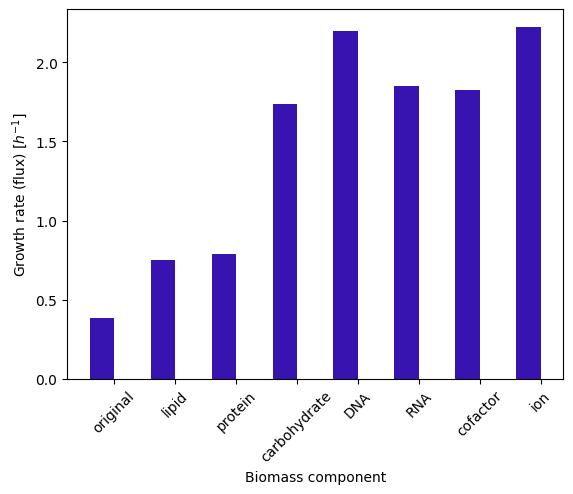
\includegraphics[width=.9\linewidth]{ablation_example_fluxes.png}
  \caption{
    Growth rates, from fluxes of the biomass reaction, from the original wild type model ($\gro$; leftmost bar) and from the ablated versions of the model ($\griabl$, where $i$ represents each biomass components among lipids, proteins, carbohydrates, DNA, RNA, cofactors, and ions; other bars)
  }
  \label{fig:model-ablate-fluxes}
\end{figure}

I get modified growth rates as in figure~\ref{fig:model-ablate-fluxes}.

\begin{figure}
  \centering
  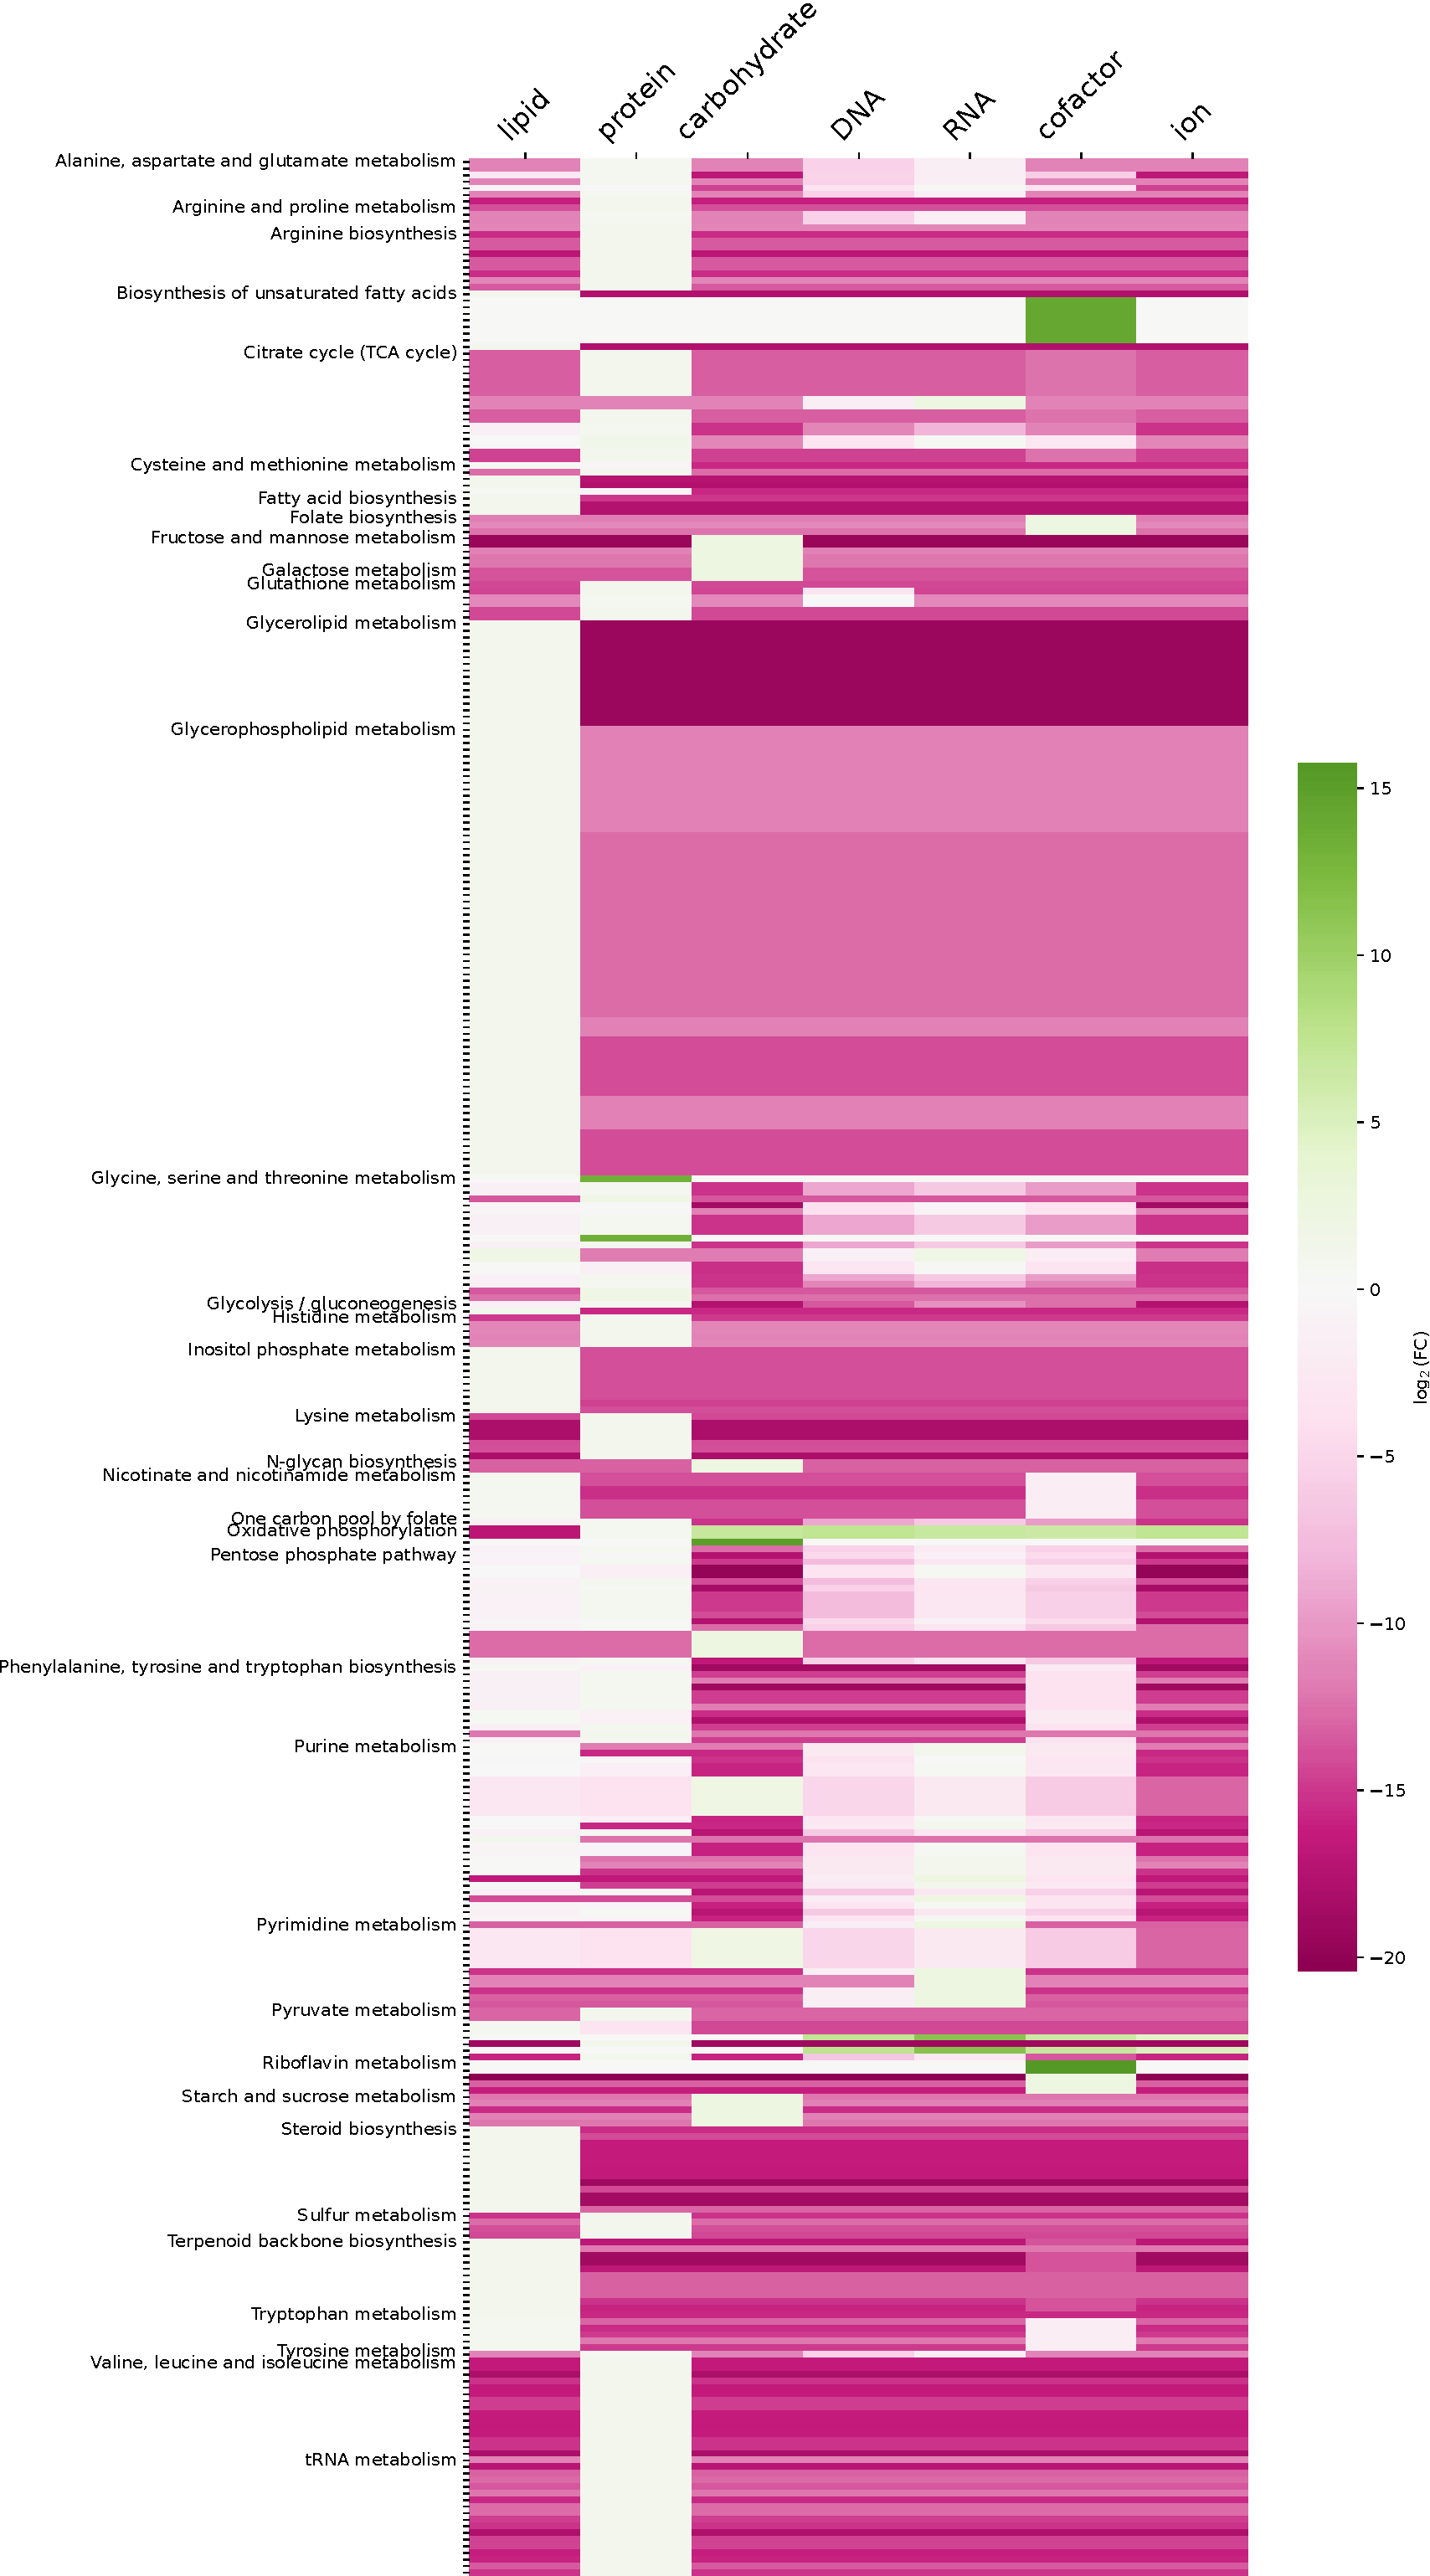
\includegraphics[width=.8\linewidth]{allocation_fc}
  \caption{
    The cell changes how it allocates its proteome to enzymes when different components of its biomass are prioritised.
    Each column shows the component that remains in each round of pseudometabolite ablation.
    Rows represent reactions, sorted by subsystem.
    Colours represent how the cell re-allocates its proteome to each enzyme: green shows an increase in reaction flux, while pink shows a decrease in flux.
    Fluxes with magnitude less than $\epsilon = $ \SI{1.11d-11}{\mmolgdw} are treated as $\epsilon$ flux, for the purpose of computing fold changes.
    Cases where $|\log_{2}(\mathrm{FC})| < 17$ are excluded to restrict the number of reactions ($n = 3897$) to aid display purposes.
  }
  \label{fig:model-ablate-enz-use}
\end{figure}

When the model prioritises a different biomass component in each round of ablation, the model partitions the limited proteome available for enzyme production differently.
In other words, in each round of ablation, the vector of fluxes carried by each enzyme usage pseudo-reaction (defined in equation~\ref{eq:model-gecko-enzyme-usage}) is different from each other and the non-ablated case.
Subsystem information provides a biologically relevant picture to these changes.
More specifically, I match the flux carried by each enzyme usage pseudo-reaction to the enzyme-catalysed reaction that the enzyme is associated with.
If an enzyme usage pseudo-reaction is associated with multiple enzyme-catalysed reactions, data entries were duplicated accordingly.
Then, the subsystem associated with each enzyme-catalysed reaction is taken.
To emphasise changes in proteome allocation across rounds of ablation, I compute the fold change of fluxes relative to the non-ablated case.
It is important to note that some reaction fluxes in some cases are zero, making the logarithm of fold change undefined.
As a workaround, I defined a threshold small flux $\epsilon = $ \SI{1.11d-11}{\mmolgdwh}, which corresponds to one molecule per cell per hour --- the reasoning being that if a reaction is important enough for the yeast cell, the cell fires the reaction more than once in an hour, which is a substantial proportion of its doubling time.
For the purposes of computing fold changes, fluxes with magnitude less than $\epsilon = $ \SI{1.11d-11}{\mmolgdw}, including zero flux, are thus treated as $\epsilon$ flux.
Therefore, extremely high ($> 10$) $\log_{2}(\mathrm{FC})$ likely indicates an original zero flux becoming non-zero in ablation, interpreted as an enzyme `switching-on', while extremely low ($< -10$) $\log_{2}(\mathrm{FC})$ likely indicates an original non-zero flux becoming zero in ablation, interpreted as an enzyme `switching-off'.
Fold changes thus indicate changing priorities for the cell: a positive $\log_{2}(\mathrm{FC})$ represents more of the proteome allocated to the production of the relevant enzyme, while a negative $\log_{2}(\mathrm{FC})$ represents less of the proteome allocated to the production of the relevant enzyme.

Figure~\ref{fig:model-ablate-enz-use} shows the subsystems and fold changes as described above.
In particular, it shows:

\begin{enumerate}
  \item In most cases, enzymes are `switched-off', though lipid-prioritised biosynthesis is most similar to the parallel case.
  \item Increased fatty acid biosynthesis, glycerolipid metabolism, glycerophospholipid metabolism, inositol phosphate metabolism, steroid biosynthesis, and terpenoid backbone biosynthesis when lipid is prioritised.
        Decreases in amino acid metabolism, which varied depending on the amino acid.
        Decreased oxidative phosphorylation and TCA cycle.
  \item Small increases in amino acid metabolism, tRNA metabolism, and oxidative phosphorylation when protein is prioritised.
        Decrease in glycine, serine, and threonine metabolism is strong in carbohydrate and ion, but weaker in DNA, RNA, and cofactor prioritisation.
  \item Increase in fructose and mannose metabolism when carbohydrate is prioritised.
        Strong increase in riboflavin metabolism when cofactor is prioritised (riboflavin is a cofactor).
        Increase in pentose phosphate pathway, purine metabolism, and pyrimidine metabolism when RNA is prioritised.
        However, decrease in pentose phosphate pathway when DNA is prioritised.
  \item For carbohydrate, DNA, RNA, cofactor, ion, strong increases in glycolysis/gluconeogenesis and oxidative phosphorylation.
\end{enumerate}

In sum, changes in allocation in rounds of ablation, by subsystem, is reasonable given the roles of the enzymes, and this visualisation confirms that the ablation is reasonable.

\section{Estimating timescale of biosynthesis}
\label{sec:model-timescale}

% Do I get the same ablation barcharts if glucose uptake is at saturation (i.e. 8.69)?
% Judging by the ratio heatmaps later in the chapter, I think the answer is no, and
% so maybe it makes sense to `max out' the glucose uptake for now.
I used the ecYeast8.6.0 model with glucose uptake, defined by the bounds of its exchange reaction flux, restricted to within \SIrange{0}{16.89}{\mmolgdw}.
The upper limit is based on the glucose uptake rate from using the non-modified model to optimise growth rate.
This value agrees with theoretical saturation rates of \SIrange{16}{19}{\mmolgdw} \parencite{blankTCACycleActivity2004}.
Using the biomass reaction as the objective function, I optimise the model to obtain the predicted growth rate, and computed the doubling time based on this growth rate as follows:

\begin{equation}
  t_{0} = \frac{\ln 2}{\gro}
  \label{eq:model-doubling-time}
\end{equation}

where $t_{0}$ is the doubling time and $\gro$ is the growth rate, equivalent to the optimal flux of the biomass reaction.

I ablate components in the biomass reaction that have pseudoreactions associated with the `Growth' subsystem, as discussed in section~\ref{sec:model-yeast8-pseudometabolites} in turn.
In each round, the model is simulated, using the modified biomass reaction as the objective function, and the flux is recorded.
Doubling time is computed, taking into account the mass fraction of each biomass component --- i.e.\ if the component is a smaller fraction of the cell, it takes less time.
Specifically, the computation is:

\begin{equation}
  \Tiabl = f_{i} \cdot \frac{\ln 2}{\griabl}
  \label{eq:model-ablated-time}
\end{equation}

where $i$ represents each of the biomass components (lipids, proteins, carbohydrates, DNA, RNA, cofactors, and ions), $\Tiabl$ is the predicted time for synthesis of each biomass component, $f_{i}$ is the mass fraction of each biomass component, and $\griabl$ is optimal flux of the ablated biomass reaction.
$f_{i}$ for each biomass component is computed by dividing the molecular weight of the corresponding pseudometabolite by the molecular weight of biomass (table~\ref{tab:ecyeast8-mol-weights}).

For comparison, I computed estimates of the time for each biomass component, assuming that it is proportional to the mass fraction:

\begin{equation}
  t_{i} = f_{i} \cdot t_{0}
  \label{eq:model-proportional-time}
\end{equation}

where $t_{0}$ is the doubling time found in equation~\ref{eq:model-doubling-time}.

\begin{figure}
  \centering
  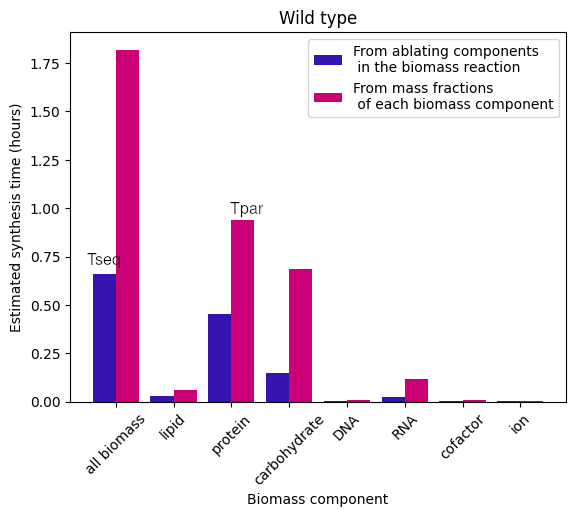
\includegraphics[width=.9\linewidth]{ablation_example_ratio.png}
  \caption{
    Comparing time scales derived from ablating components of the biomass reaction (blue) and from assuming that synthesis time is proportional to the mass fraction of the biomass component (red).
    For each biomass component (lipid, protein, carbohydrate, DNA, RNA, cofactor, ion), the time $\Tiabl$ was computed according to equation~\ref{eq:model-ablated-time} (blue bars apart from leftmost column), and the time $t_{i}$ was computed according to equation~\ref{eq:model-proportional-time} (red bars apart from leftmost column).
    $\Tpar$ is defined as the greatest $t_{i}$ (equation~\ref{eq:model-b}).
    Blue under `all biomass' is $\Tseq$ (equation~\ref{eq:model-a}), the sum of times derived from ablation (other blue bars).
    Red under `all biomass' is the doubling time $t_{0}$ (equation~\ref{eq:model-doubling-time}).
  }
  \label{fig:model-ablate-times}
\end{figure}

Figure~\ref{fig:model-ablate-times} summarises the times $t_{0}$ along with $\Tiabl$ and $t_{i}$ for each biomass component.

To determine whether sequential biosynthesis of biomass components or parallel biosynthesis of biomass components is advantageous, I devise a ratio $\ratioabl$ that represents ratio between the total time predicted by ablation and the biomass component that is predicted to take the most time is computed, i.e.\

\begin{equation}
  \ratioabl \coloneqq \frac{\Tseq}{\Tpar}
  \label{eq:model-ratio-simplified}
\end{equation}

$\Tseq$ represents sum of times from focusing on each biomass component --- thus representing time predicted, assuming biomass components are synthesised in turn:

\begin{equation}
  \Tseq \coloneqq \sum_{i} \Tiabl = \sum f_{i} \cdot \frac{\ln 2}{\griabl}
  \label{eq:model-a}
\end{equation}

$\Tpar$ represents greatest time of synthesis of the biomass component if time is assumed to be proportional to mass fraction.
This is always protein as it accounts for $\approx$50\% of the mass fraction (table~\ref{tab:ecyeast8-mol-weights}):

\begin{equation}
  \begin{aligned}
    \Tpar \coloneqq \argmax_{i} t_{i} = \Tabl{protein} = \biomfrac{protein} \cdot \frac{\ln 2}{\gro},\\
    \because \argmax_{i} f_{i} = \biomfrac{protein}
  \end{aligned}
  \label{eq:model-b}
\end{equation}

$\Tpar$ thus represents the limiting, slowest process.

Therefore,

\begin{equation}
  \begin{aligned}
    \ratioabl &= \frac{\Tseq}{\Tpar} \\
    & = (\sum_i \frac{f_i}{\griabl}) \cdot \frac{\gro}{\biomfrac{protein}} \\
    & = (\frac{\biomfrac{lipid}}{\grabl{lipid}} + \frac{\biomfrac{protein}}{\grabl{protein}} + \ldots + \frac{\biomfrac{ion}}{\grabl{ion}}) \cdot \frac{\gro}{\biomfrac{protein}}
    \end{aligned}
  \label{eq:model-ratio}
\end{equation}

This expression means that the definition of the $\ratioabl$ ratio is not trivial and depends on the $\gro$ and the $\griabl$ values, which are all independent of each other.
This relationship between $\ratioabl$ and $\gro$ and $\griabl$ is further explored in section~\ref{sec:model-pool}.

\begin{figure}
  \centering
  \begin{subfigure}[htpb]{0.45\textwidth}
   \centering
   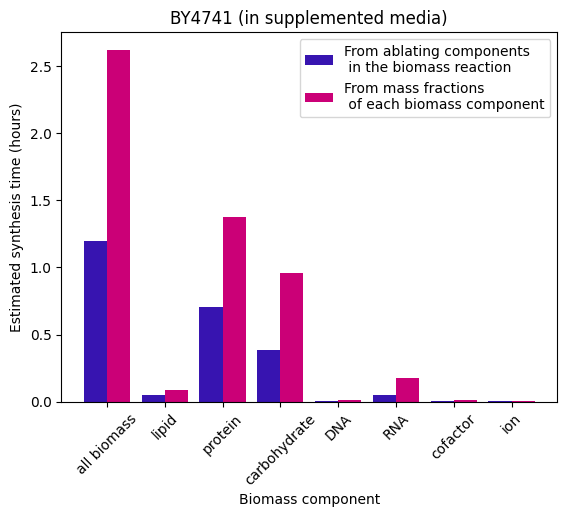
\includegraphics[width=\textwidth]{ablation_by4741}
   \caption{
     BY4741
   }
   \label{fig:model-ablation-by4741}
  \end{subfigure}
  \begin{subfigure}[htpb]{0.45\textwidth}
   \centering
   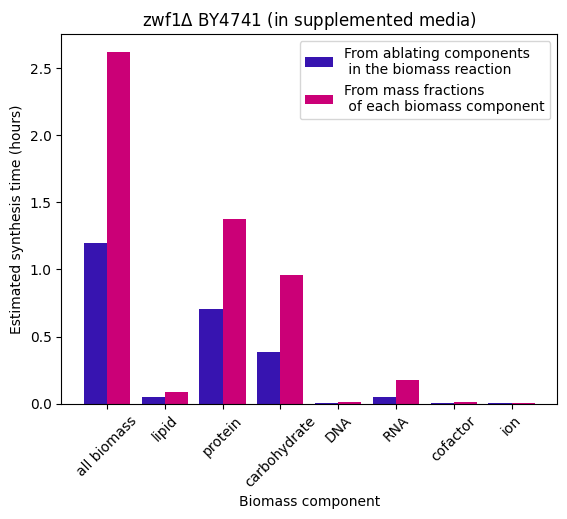
\includegraphics[width=\textwidth]{ablation_zwf1}
   \caption{
     zwf$\Delta$ in the BY4741 background.
   }
   \label{fig:model-ablation-zwf1}
  \end{subfigure}
  \begin{subfigure}[htpb]{0.45\textwidth}
   \centering
   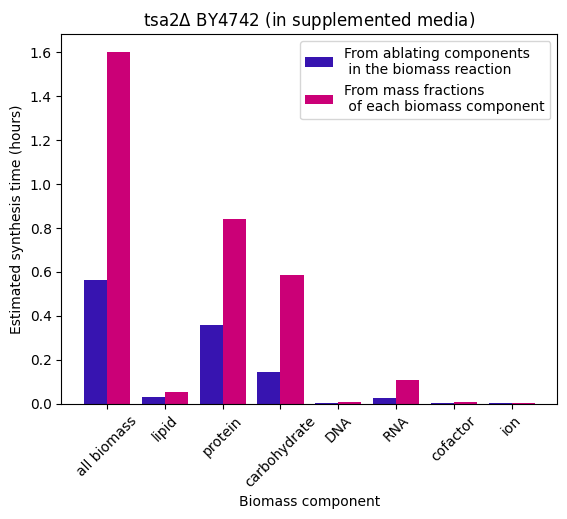
\includegraphics[width=\textwidth]{ablation_tsa2}
   \caption{
     tsa2$\Delta$ in the BY4742 background.  The ecYeast8 model does not include reactions that correspond to \textit{TSA1}.
   }
   \label{fig:model-ablation-tsa2}
  \end{subfigure}
  \caption{
    Comparing time scales from sequential and parallel biosynthesis in auxotrophs and deletion strains, as in figure~\ref{fig:model-ablate-times}.
    For BY4741-background strains, supplements are simulated by allowing uptake of histidine, leucine, tryptophan, methionine and uracil.
    The same applied to BY4742-background strains, but lysine uptake replaces methionine uptake.
  }
  \label{fig:model-ablation-strains}
\end{figure}
% Adding supplements, e.g. amino acids, dNTPs/NTPs, pyruvate, glucose limitation?
% Or do C/N grid heatmaps demonstrate this.

$\ratioabl < 1$ means that synthesising biomass components in sequence saves more time, while $\ratioabl > 1$ indicated that parallel synthesis of biomass components is favoured as synthesising biomass components in sequence does not save time.
In figure~\ref{fig:model-ablate-times}, the ratio is 0.70.
The fact that this still holds true for auxotrophs and deletion strains supports experimental evidence that auxotrophs and deletion strains have YMCs (figure~\ref{fig:model-ablation-strains}).

\section{Effect of restricting the enzyme pool}
\label{sec:model-pool}

Evaluating the hypothesis of whether a restriction of the proteome pool favours sequential biosynthesis of biomass components has multiple approaches.
Here, I discuss three commonly-used approaches --- parsimonious FBA, regularised FBA, and constraining the sum of absolute values of fluxes --- before justifying the use of directly varying a parameter in the ecYeast8 model to take advantage of GECKO.

Parsimonious FBA \parencite{lewisOmicDataEvolved2010} first uses FBA to compute optimal growth rate, fixes this value, then minimises the sum of gene-associated reaction fluxes while maintaining optimal growth.
Depending on the software package, this minimisation either minimises the sum of fluxes (COBRA, for MATLAB), the sum of the absolute values of each flux (\textit{cobrapy}, for the Python programming language) or squared sum (COBREXA, for the Julia programming language).
I reject this approach because it fixes the growth rate, but I aim to see how constraints affect cell strategies as the constraints vary along a spectrum.
Additionally, parsimonious FBA relies on reducing the subset of genes that contribute to the solution.
In other words, it modifies the model and it also relies on good gene-protein annotations, the latter not being a guarantee.

Regularised FBA is defined as adding a regularisation parameter to the objective function.
\textcite{vijayakumarHybridFluxBalance2020} describe a quadratic program for solving a regularised two-level FBA:

\begin{equation}
  \max g^\intercal v - \frac{\sigma}{2}v^\intercal v
  \label{eq:model-regularised-fba}
\end{equation}

where $g$ is the objective function, $v$ is the flux vector, and $\sigma$ is a regularisation parameter than can be tuned.

I reject this approach because it requires a quadratic solver, making it difficult and computationally expensive to implement.
% Add figure to show this unexpected behaviour?
And because the behaviour is not as expected, i.e.\ the growth rate does not change as the regularisation parameter $\sigma$ varies, even though I expected a trade-off between growth and reaction fluxes to change as this parameter varies.

Constraining the sum of absolute values of fluxes is simply defined as fixing

\begin{equation}
  \sum_{i} |v_{i}| < c
  \label{eq:model-constrain-sumfluxes}
\end{equation}

where $v_{i}$ represents each flux of each reaction, and $c$ is a constant to be varied.

This is reasonable for the original Yeast8 model without the enzyme constraint, as opposed to ecYeast8.
% ADD PLOTS TO SHOW THIS?
As $c$ decreases to 0, the original growth rate $\gro$ and ablated growth rates $\griabl$ decreased to 0 linearly, while the $\ratioabl$ ratio remains constant.
However, if this approaches is applied to ecYeast8,
there is potential triple-counting of imposing constraints, i.e.\: additionally on
(a) constraints on enzyme usage imposed on the enzyme-usage pseudoreactions created by GECKO, and on
(b) constraints on sum of the absolute values of fluxes.
This will confuse interpretation.

Therefore, I decide to vary $\epool$ to study proteomic constraints as this takes advantage of a formalism that already exists in ecYeast8, by virtue of GECKO, that is easy to interpret and modify.

\begin{figure}
  \centering
  \begin{subfigure}[htpb]{0.45\textwidth}
   \centering
   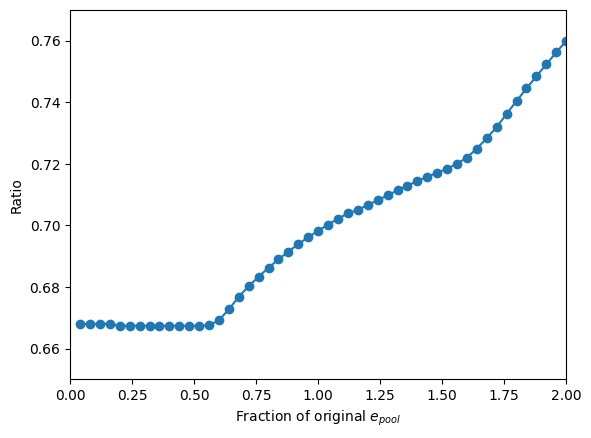
\includegraphics[width=\textwidth]{epool_ec_ratio_shrinkyaxis}
   \caption{
     Effect on ratio ($\ratioabl$), $\epool^{\prime} \leq 2\epool$.
   }
   \label{fig:model-pool-ratio}
  \end{subfigure}%
  \begin{subfigure}[htpb]{0.45\textwidth}
   \centering
   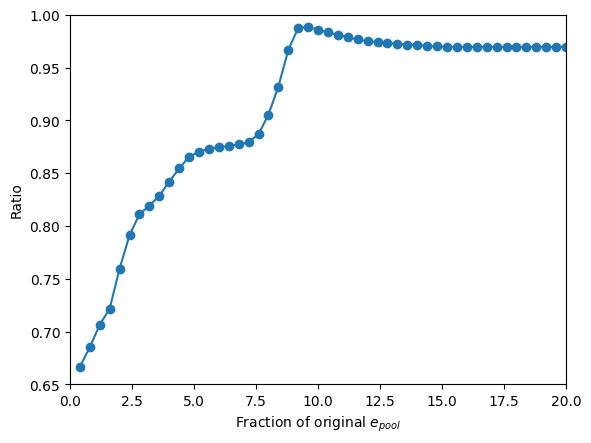
\includegraphics[width=\textwidth]{epool_ec_ratio_20_shrinkyaxis}
   \caption{
     Effect on ratio ($\ratioabl$), $\epool^{\prime} \leq 20\epool$.
   }
   \label{fig:model-pool-ratio-20}
  \end{subfigure}

  \begin{subfigure}[htpb]{0.45\textwidth}
   \centering
   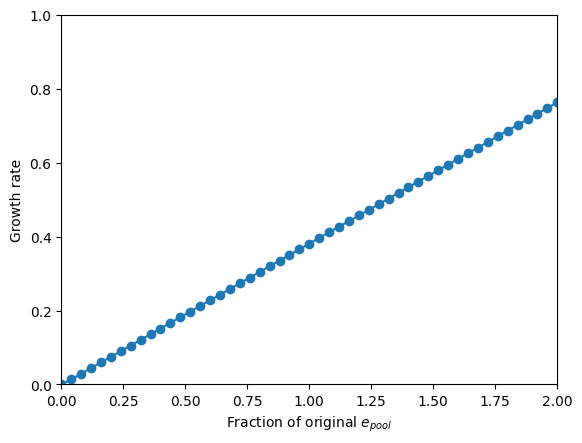
\includegraphics[width=\textwidth]{epool_ec_gr}
   \caption{
     Effect on wild type growth rate ($\gro$), $\epool^{\prime} \leq 2\epool$.
   }
   \label{fig:model-pool-growthrate}
  \end{subfigure}%
  \begin{subfigure}[htpb]{0.45\textwidth}
   \centering
   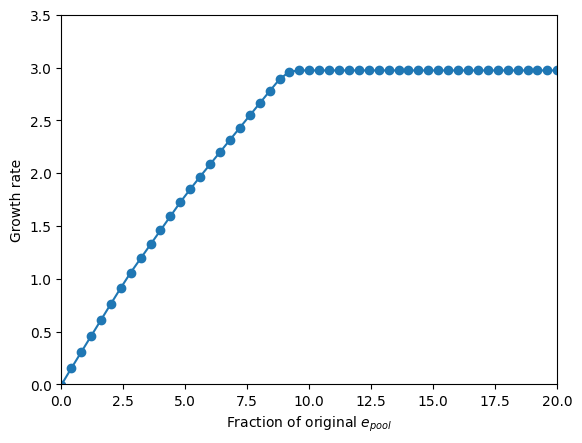
\includegraphics[width=\textwidth]{epool_ec_gr_20}
   \caption{
     Effect on wild type growth rate ($\gro$), $\epool^{\prime} \leq 20\epool$.
   }
   \label{fig:model-pool-growthrate-20}
  \end{subfigure}

  \begin{subfigure}[htpb]{0.45\textwidth}
   \centering
   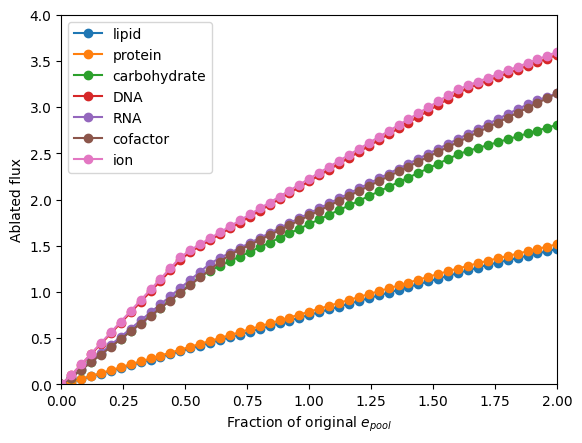
\includegraphics[width=\textwidth]{epool_ec_components}
   \caption{
     Effect on ablated growth rates ($\griabl$), $\epool^{\prime} \leq 2\epool$.
   }
   \label{fig:model-pool-ablated}
  \end{subfigure}%
  \begin{subfigure}[htpb]{0.45\textwidth}
   \centering
   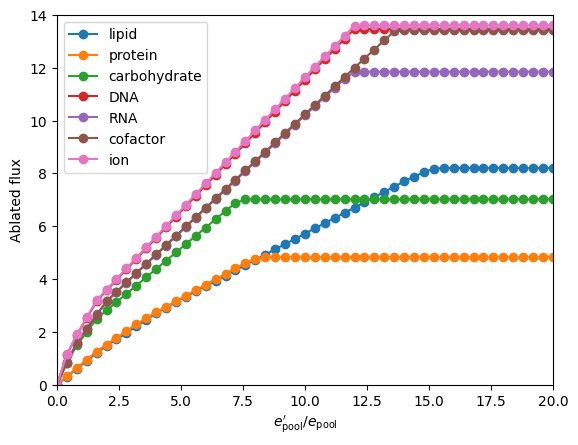
\includegraphics[width=\textwidth]{epool_ec_components_20}
   \caption{
     Effect on ablated growth rates ($\griabl$), $\epool^{\prime} \leq 20\epool$.
   }
   \label{fig:model-pool-ablated-20}
  \end{subfigure}

  \caption{
    Constraining the proteome pool available for synthesis enzymes (decreasing $\epool$) leads to a greater advantage of sequential biosynthesis of biomass components over parallel biosynthesis, as evidenced by a decreasing $\ratioabl$ ratio (\ref{fig:model-pool-ratio}).
    Concurrently, the wild type growth rate ($\gro$) decreases linearly to zero (\ref{fig:model-pool-growthrate}) and ablated growth rates ($\griabl$) decrease in linear segments independently of each other and of the growth rate (\ref{fig:model-pool-growthrate}); these values determine the ratio according to equation~\ref{eq:model-ratio}.
  }
  \label{fig:model-pool}
\end{figure}

To vary the enzyme-available proteome pool in the ecYeast8 model,
I vary the value of the upper limit of the flux $\epool$ of the enzyme pool pseudoreaction (equation~\ref{eq:model-gecko-enzyme-pool}) in order to change the flux available for enzyme usage pseudoreactions (equation~\ref{eq:model-gecko-enzyme-pool}).
The logic of this is that with a smaller $\epool$, the sum total of fluxes of the enzyme usage pseudoreactions must decrease, and the model must decide which enzyme usage pseudoreactions to allocate a higher flux to.
This models the biological situation in which the cell has a smaller enzyme-available proteome pool, so the cell must decide which enzymes to allocate the greatest proportions of the pool to.

Figure~\ref{fig:model-pool} shows the results of my investigation.
I denote $\epool$ as the default enzyme-available proteome pool (INSERT EXACT VALUE HERE) and $\epool^{\prime}$.
When $0 \leq \epool^{\prime} \leq 2\epool$, the model gives realistic growth rates \SIrange{0}{0.8}{\hour^{-1}} (figure~\ref{fig:model-pool-growthrate}).
In this region, growth rate varies linearly as $\epool$ varies.
With higher $\epool^{\prime}$ values --- that is, less of a constraint on the enzyme pool --- the ratio increases, indicating less advantage for sequential biosynthesis (figure~\ref{fig:model-pool-ratio}).
As $\epool^{\prime}$ increases, ablated growth rates $\griabl$ increases linearly at low $\epool^{\prime}$ (figure~\ref{fig:model-pool-ablated}).
But then, at higher $\epool^{\prime}$, these linear relationships decrease in gradient, all going to a plateau at very high $\epool^{\prime}$ (figure~\ref{fig:model-pool-ablated-20}).
This behaviour shows that the relationship between $\griabl$ and $\epool^{\prime}$ is independent of the growth rate $\gro$ and of each other.
% TODO: Come up with a better (biological) interpretation -- consult some org notes.
Different components plateau at different $\epool^{\prime}$, with carbohydrate reaching a plateau first, followed by protein.
This may indicate that the enzyme-available proteome pool is limiting for these components, which may be because they are more `expensive' in terms of the amount of protein needed for the synthesis of related enzymes.

To explain the increase in $\ratioabl$ as $\epool^{\prime}$ increases, I consider the behaviour of $\gro$ and $\griabl$ values with respect to $\epool^{\prime}$ in intervals.
As a simplification, I express the size of $\epool^{\prime}$ in multiples of the original $\epool$ and denote the size of $\epool^{\prime}$ as $x$.

Let $\ratioabl$, given by equation~\ref{eq:model-ratio}, depend on $x$:

\begin{equation}
  \label{eq:model-ratio-x}
  \ratioabl(x) = \left( \sum_i \frac{f_i}{\griabl(x)} \right) \cdot \frac{\gro(x)}{\biomfrac{protein}}
\end{equation}

This expression takes into account how $\gro$ and $\griabl$ values vary with $x$, and how $f_{i}$ values are constants.

We thus obtain:
\begin{equation}
  \begin{aligned}
  \ndif{\ratioabl(x)}{x} &= \frac{1}{\biomfrac{protein}} \ndif{}{x} \left[ \left( \sum_i \frac{f_i}{\griabl(x)} \right) \cdot \gro(x) \right]\\
  &= \frac{1}{\biomfrac{protein}} \left[ \left( \sum_i \frac{f_i}{\griabl(x)} \right) \cdot \ndif{\gro(x)}{x} + \gro(x) \ndif{}{x} \left( \sum_i \frac{f_i}{\griabl(x)} \right) \right]\\
  &= \frac{1}{\biomfrac{protein}} \left[ \left( \sum_i \frac{f_i}{\griabl(x)} \right) \cdot \ndif{\gro(x)}{x} - \gro(x) \sum_{i}\left( \frac{f_{i}}{\griabl(x)^{2}} \cdot \ndif{\griabl(x)}{x} \right) \right]
  \end{aligned}
  \label{eq:model-ratio-diff}
\end{equation}

Consider $0 \leq x \leq 0.5$.
In this region of $x$, let $\gro = k_{0}x$ and $\griabl = k_{i}x$, where constants $k_{0}, k_{i} > 0$.
This models observations in figure~\ref{fig:model-pool}.
Equation~\ref{eq:model-ratio-diff} thus becomes:
\begin{equation}
  \begin{aligned}
  \ndif{\ratioabl(x)}{x} &= \frac{1}{\biomfrac{protein}} \left[ \left( \sum_i \frac{f_i}{k_{i}x} \right) \cdot k_{0} - k_{0}x \sum_{i}\left( \frac{f_{i}}{(k_{i}x)^{2}} \cdot k_{i} \right) \right]\\
  &= \frac{1}{\biomfrac{protein}} \left[ \frac{k_{0}}{x} \sum_i \frac{f_i}{k_{i}} - k_{0}x \left( \sum_{i} \frac{f_{i}}{k_{i}x^{2}} \right) \right]\\
  &= \frac{1}{\biomfrac{protein}} \left[ \frac{k_{0}}{x} \sum_i \frac{f_i}{k_{i}} - \frac{k_{0}}{x} \sum_i \frac{f_i}{k_{i}} \right]\\
  &= 0
  \end{aligned}
  \label{eq:model-ratio-diff-smallx}
\end{equation}

And this explains the constant $\ratioabl$ in this region.

Now, consider $0.5 < x \leq 9$.
In this region, the trajectories of $\griabl$ with respect to time remain linear, but some with changes in slope.
In other words, in a sub-region where the slopes of all $\griabl$ are constant, we can let: $\gro = k_{0}x$ and $\griabl = m_{i}x + c_{i}$, where $k_{0}, m_{i}, c_{i} > 0$.
Equation~\ref{eq:model-ratio-diff} thus becomes:
\begin{equation}
  \begin{aligned}
  \ndif{\ratioabl(x)}{x} &= \frac{1}{\biomfrac{protein}} \left[ \left( \sum_i \frac{f_i}{m_{i}x+c_{i}} \right) \cdot k_{0} - k_{0}x \sum_{i}\left( \frac{f_{i}}{(m_{i}x+c_{i})^{2}} \cdot m_{i} \right) \right]\\
  &= \frac{k_{0}}{\biomfrac{protein}} \left[ \left( \sum_i \frac{f_i}{m_{i}x+c_{i}} \right) - x \left( \sum_{i} \frac{f_{i}m_{i}}{(m_{i}x+c_{i})^{2}} \right) \right]\\
  &= \frac{k_{0}}{\biomfrac{protein}} \sum_{i} \left[ \frac{f_i}{m_{i}x+c_{i}} - \frac{xf_{i}m_{i}}{(m_{i}x+c_{i})^{2}} \right]\\
  &= \frac{k_{0}}{\biomfrac{protein}} \sum_{i} \left[ \frac{f_{i}c_{i}}{(m_{i}x+c_{i})^{2}} \right]
  \end{aligned}
  \label{eq:model-ratio-diff-midx}
\end{equation}

As $f_{i}, c_{i}, m_{i} > 0$ for all biomass components $i$, and $k_{0} > 0$, $\ndif{\ratioabl(x)}{x} > 0$ regardless of the specific values that these constants take.
Because $k_{0}$ does not change over the region of $x$ considered, $m_{i}$, $c_{i}$, and $x$ values thus determine the magnitude of $\ndif{\ratioabl(x)}{x}$.
If within a region of $x$, $m_{i}$ and $c_{i}$ values remain constant for all $i$, then as $x$ increases, $\ndif{\ratioabl(x)}{x}$ should decrease --- this is certainly the case, as can be observed in figure~\ref{fig:model-pool}.

Lastly, consider $x > 9$.
In this region, $\gro$ becomes constant, thus we let $\gro = k_{0}$.
We keep $\griabl = m_{i}x + c_{i}$, and as before, $k_{0}, m_{i}, c_{i} > 0$.
Equation~\ref{eq:model-ratio-diff} thus becomes:
\begin{equation}
  \begin{aligned}
  \ndif{\ratioabl(x)}{x} &= \frac{1}{\biomfrac{protein}} \left[ 0 - k_{0} \sum_{i}\left( \frac{f_{i}}{(m_{i}x+c_{i})^{2}} \cdot m_{i} \right) \right]\\
  &= -\frac{k_{0}}{\biomfrac{protein}} \sum_{i}\left[ \frac{f_{i}m_{i}}{(m_{i}x+c_{i})^{2}} \right]
  \end{aligned}
  \label{eq:model-ratio-diff-largex}
\end{equation}

This predicts \emph{decreasing} $\ratioabl$ as $x$ increases in this region.
Because $k_{0}$ is constant in this region, the rate of this decrease is thus controlled by $m_{i}$ and $c_{i}$ values.
As each $\griabl$ trajectory becomes flat as $x$ increases, each $\frac{f_{i}m_{i}}{(m_{i}x+c_{i})^{2}}$ term becomes zero, thus shrinking the magnitude of $\ndif{\ratioabl(x)}{x}$.
Finally, as all $\griabl$ trajectories become flat at $x > 15$, $\ndif{\ratioabl(x)}{x} = 0$.


\section{Effect of carbon and nitrogen sources}
\label{sec:model-exchange}

\subsection{Exchange reaction saturation}
\label{subsec:model-saturation}

FBA models include nutrient exchange reactions to simulate the presence of certain nutrients in the growth medium.
Because FBA models do not account for substrate concentrations, studying the effect of nutrient sources in FBA models involves constraining the flux of such exchange reactions to achieve validated growth rates, as performed by \textcite{elsemmanWholecellModelingYeast2022} to study the effect of glucose.

Using the ecYeast8.6.0 model, I varied the flux bounds of exchange reaction and recorded how it affects predicted growth rate.
I did this with two carbon sources, glucose and pyruvate, and with ammonium as a nitrogen source (figure~\ref{fig:model-saturation}).

% TODO: Remove the right panel figs
\begin{figure}
  \centering
  \begin{subfigure}[t]{0.45\textwidth}
  \centering
    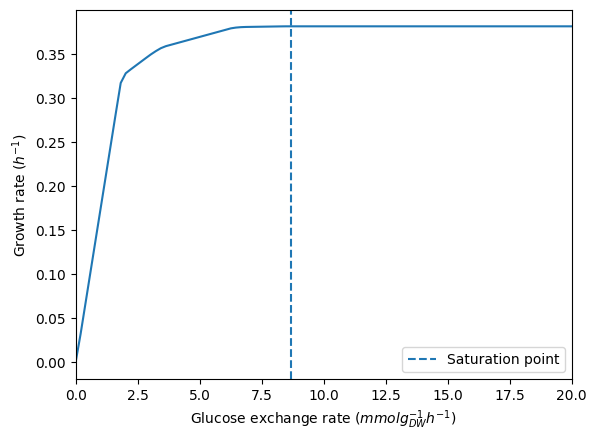
\includegraphics[width=\linewidth]{saturation_glc}
    \caption{
      Effect of glucose exchange on growth rate, with ammonium exchange flux unrestricted.
      Growth rate saturation is at \SI{8.69}{\mmolgdwh}.
    }
    \label{fig:model-saturation-glucose}
  \end{subfigure}%
  \begin{subfigure}[t]{0.45\textwidth}
  \centering
    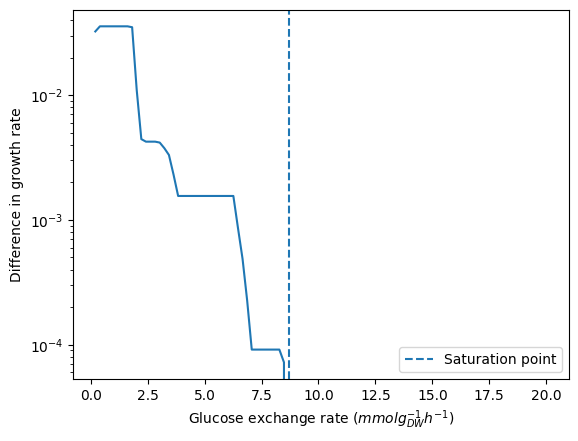
\includegraphics[width=\linewidth]{saturation_diff_glc}
    \caption{
    }
    \label{fig:model-saturation-diff-glucose}
  \end{subfigure}

  \begin{subfigure}[t]{0.45\textwidth}
  \centering
    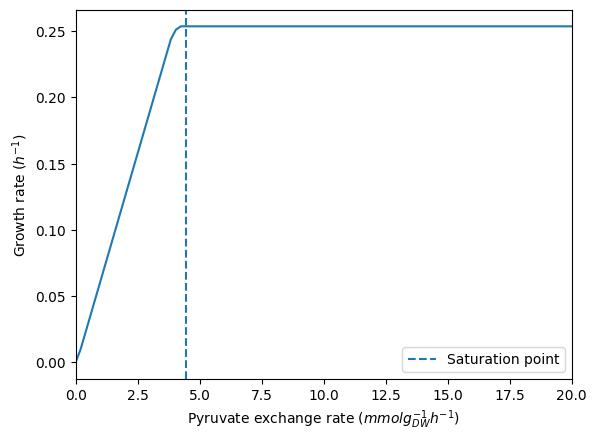
\includegraphics[width=\linewidth]{saturation_pyr}
    \caption{
      Effect of pyruvate exchange on growth rate, with ammonium exchange flux unrestricted.
      Growth rate saturation is at \SI{4.44}{\mmolgdwh}.
    }
    \label{fig:model-saturation-pyruvate}
  \end{subfigure}%
  \begin{subfigure}[t]{0.45\textwidth}
  \centering
    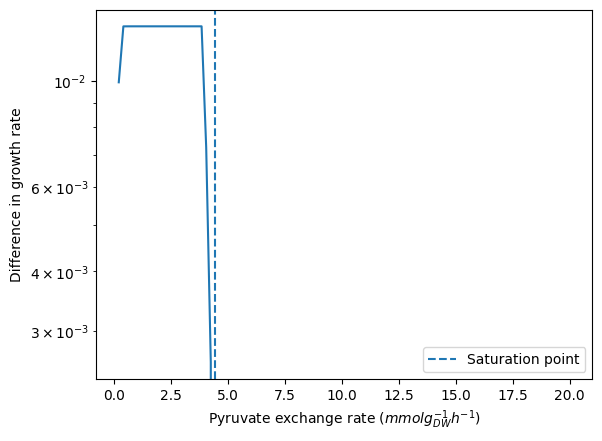
\includegraphics[width=\linewidth]{saturation_diff_pyr}
    \caption{
    }
    \label{fig:model-saturation-diff-pyruvate}
  \end{subfigure}

  \begin{subfigure}[t]{0.45\textwidth}
  \centering
    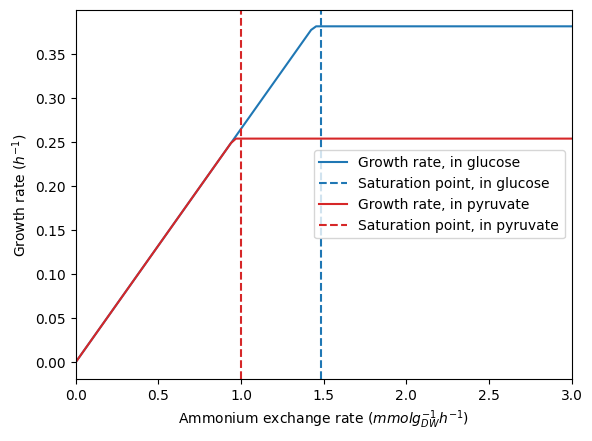
\includegraphics[width=\linewidth]{saturation_amm}
    \caption{
      Effect of ammonium exchange on growth rate, with exchanges of carbon sources set to growth rate saturation based on figures~\ref{fig:model-saturation-glucose} and ~\ref{fig:model-saturation-pyruvate}.
      Growth rate saturation is at \SI{1.48}{\mmolgdwh} in glucose, and
      at \SI{1.00}{\mmolgdwh} in pyruvate.
    }
    \label{fig:model-saturation-ammonium}
  \end{subfigure}%
  \begin{subfigure}[t]{0.45\textwidth}
  \centering
    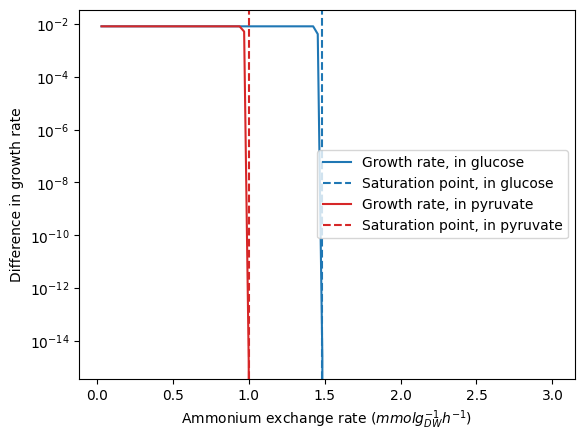
\includegraphics[width=\linewidth]{saturation_diff_amm}
    \caption{
    }
    \label{fig:model-saturation-diff-ammonium}
  \end{subfigure}

  \caption{
    Effect of nutrient exchange reactions on growth rate, predicted by the ecYeast8 model (left panels).
    Saturation values were found by computing discrete differences of growth rates with respect to exchange rates
    (right panels \ref{fig:model-saturation-diff-glucose},~\ref{fig:model-saturation-diff-pyruvate},~\ref{fig:model-saturation-diff-ammonium}),
    and saturation was termed as where the differences dropped below a small tolerance value $\epsilon = \num{1e-8}$.
  }
  \label{fig:model-saturation}
\end{figure}

The glucose saturation curve (figure~\ref{fig:model-saturation-glucose}) is similar to that predicted by \textcite{elsemmanWholecellModelingYeast2022} using another derivative of the Yeast8 model.
The saturation point is well below the maximal glucose consumption rate of \SIrange{16}{19}{\mmolgdwh} as determined by GC-MS-based metabolic flux ratio analysis \parencite{blankTCACycleActivity2004}.
In addition, the saturation curves show that the maximum growth rate on glucose is \SI{0.38}{\hour^{-1}} while the maximum growth rate on pyruvate is \SI{0.25}{\hour^{-1}} (figure~\ref{fig:model-saturation-pyruvate}).
The glucose value agrees with \textcite{domenzainReconstructionCatalogueGenomescale2022}, which uses GECKO 2, the latest published version of GECKO, to create the ecYeast7 model to predict maximum growth rates on various carbon sources, and also agrees with my experimental observations.
This paper did not predict growth rate on pyruvate, but a lower maximum growth rate on a non-fermentable carbon source compared to glucose agrees with the biochemical basis and is also consistent with my experimental observations.
Finally, the growth rate saturation point for ammonium is determined by the maximal growth rate determined by each carbon source (figure~\ref{fig:model-saturation-ammonium}).
For my subsequent investigation of the effect of carbon and nitrogen sources on the model, I use the exchange rates found in this investigation as saturation values.

\subsection{Effect of carbon and nitrogen sources on biomass synthesis strategies}
\label{subsec:model-grid}

\begin{figure}
  \centering
  \begin{subfigure}[t]{0.45\textwidth}
  \centering
    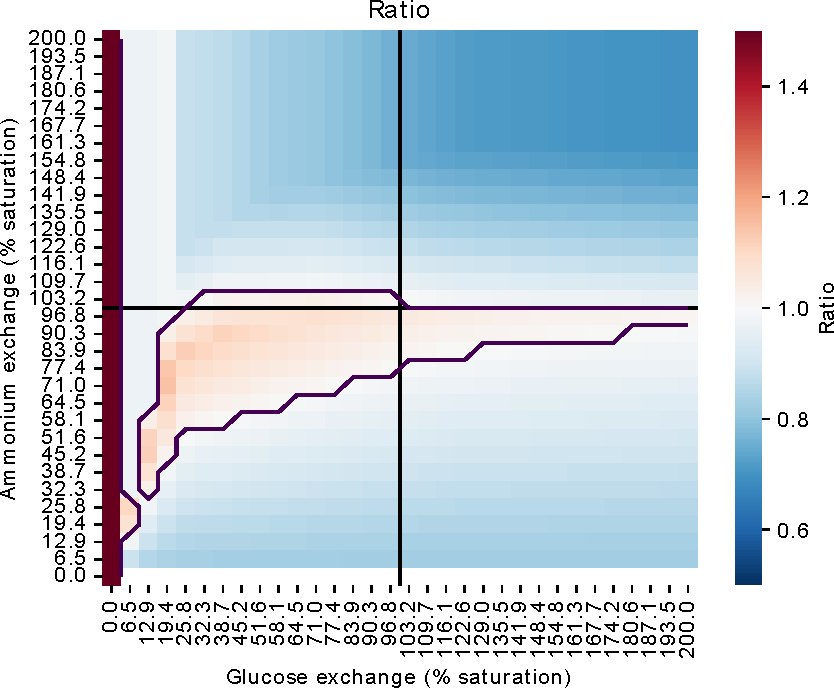
\includegraphics[width=\linewidth]{ec_grid_glc_amm_ratio}
    \caption{
      Ratio ($\ratioabl$)
    }
    \label{fig:model-grid-glc-ratio}
  \end{subfigure}%
  \begin{subfigure}[t]{0.45\textwidth}
  \centering
    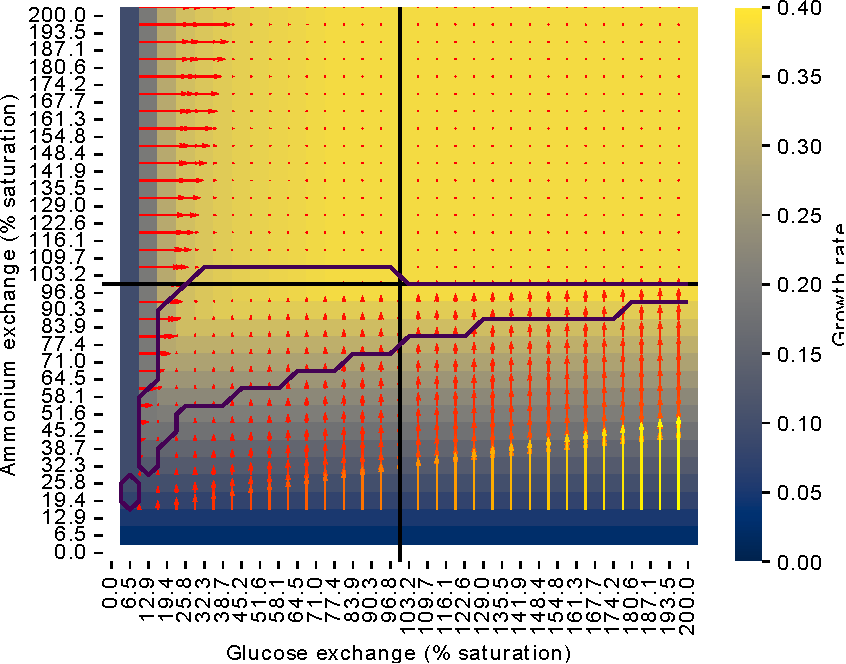
\includegraphics[width=\linewidth]{ec_grid_glc_amm_gr}
    \caption{
      Growth rate based on unmodified biomass reaction ($\gro$)
    }
    \label{fig:model-grid-glc-growthrate}
  \end{subfigure}

  \begin{subfigure}[t]{0.45\textwidth}
  \centering
    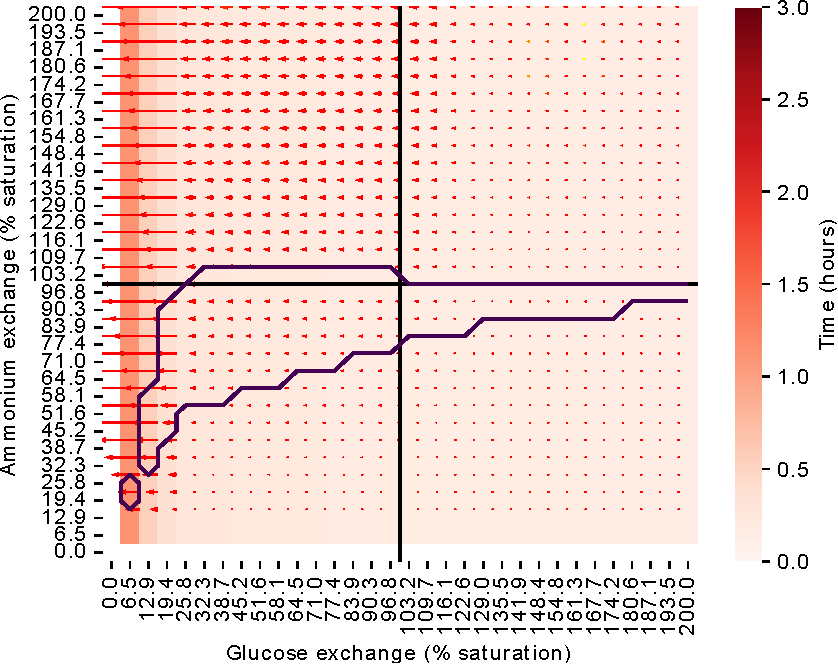
\includegraphics[width=\linewidth]{ec_grid_glc_amm_carb}
    \caption{
      $\Tabl{carbohydrate}$
    }
    \label{fig:model-grid-glc-carb}
  \end{subfigure}%
  \begin{subfigure}[t]{0.45\textwidth}
  \centering
    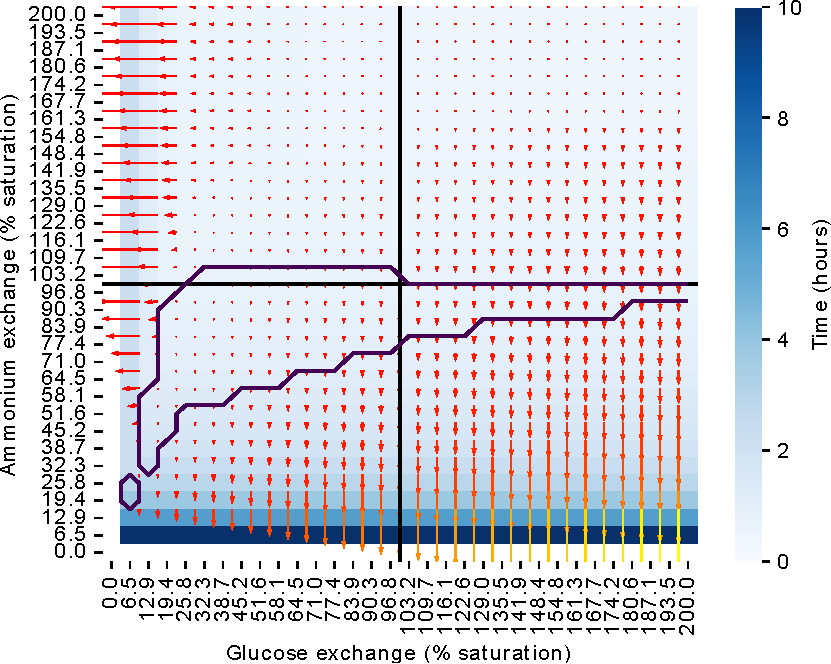
\includegraphics[width=\linewidth]{ec_grid_glc_amm_prot}
    \caption{
      $\Tabl{protein}$
    }
    \label{fig:model-grid-glc-prot}
  \end{subfigure}

  \begin{subfigure}[t]{0.45\textwidth}
  \centering
    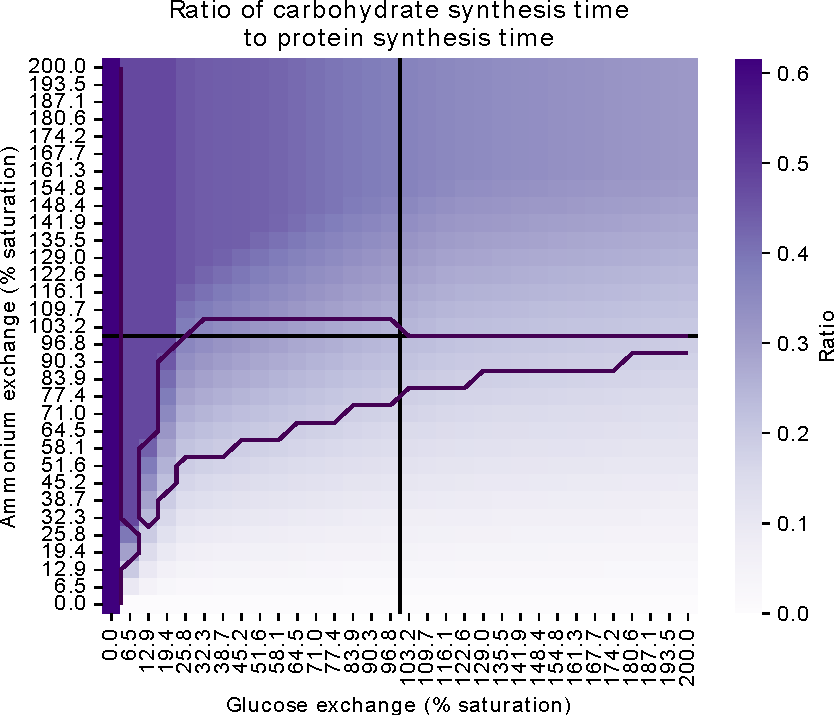
\includegraphics[width=\linewidth]{ec_grid_glc_amm_carb_to_prot}
    \caption{
      $\Tabl{carbohydrate}/\Tabl{protein}$
    }
    \label{fig:model-grid-glc-carb-to-prot}
  \end{subfigure}
  \caption{
    Effect of glucose ($\exchrate{glucose}$) and ammonium exchange rates ($\exchrate{ammonium}$) on various quantities.
    Exchange rates are expressed in percentages of growth saturation values shown in~\ref{fig:model-saturation}: glucose saturation being at \SI{8.69}{\mmolgdwh} and ammonium saturation being at \SI{1.48}{\mmolgdwh}.
    Black straight lines indicate saturation values.
    Contours show region in which ratio $\ratioabl > 1$.
    Arrows indicate susceptibility of the quantity displayed in the heatmap, relative to $\exchrate{glucose}$ and $\exchrate{ammonium}$.
  }
  \label{fig:model-grid-glc}
\end{figure}

To assess the effect of carbon and nitrogen sources on biomass synthesis strategies, I first varied the upper flux bounds of exchange reactions that correspond to glucose exchange ($\exchrate{glucose}$) and ammonium exchange rate ($\exchrate{ammonium}$).
Each of these bounds took 32 values from 0\% to 200\% saturation, with glucose saturation being at \SI{8.69}{\mmolgdwh} and ammonium saturation being at \SI{1.48}{\mmolgdwh}, to produce a grid of \num{1024} conditions.
At each combination of glucose and ammonium exchange, I ablated components in the biomass reaction according to section~\ref{sec:model-timescale} to obtain $\ratioabl$, $\gro$, $\Tabl{carbohydrate}$, and $\Tabl{protein}$.
$\ratioabl$ indicated whether the sequential or parallel strategy is advantageous for each condition, while $\gro$ indicated which nutrient source was limiting in each condition.
Synthesis times $\Tiabl$ were computed to assess whether the ratio between the synthesis times differed in different conditions, especially if the parallel biomass synthesis is favoured ($\ratioabl > 1$).
Specifically, I chose carbohydrate and protein synthesis times within $\Tiabl$ because:

\begin{enumerate}
  \item Predicted synthesis times of these biomass components varied the most, of all biomass components, as the glucose and ammonium exchange rates were varied.
  \item Each accounts for a large proportion of total biomass: protein accounts for 52.5\% and carbohydrate accounts for 36.4\% (table~\ref{tab:ecyeast8-mol-weights}).
  \item Carbohydrate synthesis has a clear biochemical relationship with a fermentable or non-fermentable carbon source.
        And, because amino acids contain amino groups, protein synthesis has a biochemical relationship with ammonium as a nitrogen source.
\end{enumerate}

And thus the ratio $\frac{\Tabl{carbohydrate}}{\Tabl{protein}}$ serves as the principal measure to quantify how biomass synthesis times change as carbon and nitrogen source concentrations change, particularly in relation to sequential biosynthesis-favouring conditions and to parallel biosynthesis-favouring conditions.

To determine whether the carbon or nitrogen source is limiting for each of the quantities calculated, I computed the susceptibility of the quantity with respect to each axis, carbon source or nitrogen source.
Susceptibility with respect to each axis is given by:

\begin{equation}
  s_{i} = \frac{R_{i}}{y} \cdot \ndif{y}{R_{i}}
  \label{eq:model-susceptibility}
\end{equation}

where $i$ indicates the axis, $y$ is the quantity of interest ($\ratioabl$, $\gro$, $\Tabl{carbohydrate}$, $\Tabl{protein}$, or $\frac{\Tabl{carbohydrate}}{\Tabl{protein}}$) at each condition, and $R_{i}$ is the exchange rate --- in this case, either $\exchrate{glucose}$ or $\exchrate{ammonium}$.

For computational use, the values of $R_{i}$ are equally-spaced discrete values from a vector with an interval $\Delta R_{i}$, and therefore the differential is approximated by central differences, given by the general formula:

\begin{equation}
  f_{i}^{\prime}(x) \approx \frac{\delta_{h}[f](x)}{2h} = \frac{f(x+h) - f(x-h)}{2h}
  \label{eq:model-central-difference}
\end{equation}

where $f$ is the function of interest and $h$ is the interval size.

Susceptibility gives an advantage over simply computing the differential of the quantity of interest with respect to the exchange rate, i.e. $\ndif{y}{R_{i}}$, because it accounts for the changing magnitude of $R_{i}$.
At greater values of $R_{i}$, the susceptibility is decreased by a greater value with respect to $\ndif{y}{R_{i}}$.
This accounts for how at such greater values of $R_{i}$, the proportional change in $R_{i}$ as it is increased or decreased by one step $\Delta R_{i}$ is smaller.

At a specific nutrient condition, if $s_{\mathrm{glucose}} > s_{\mathrm{ammonium}}$ for a quantity of interest, then it means that the quantity is more susceptible to --- or limited by --- glucose exchange at this condition.
The reverse is true if $s_{\mathrm{glucose}} < s_{\mathrm{ammonium}}$.
To visualise the extent to which either exchange rate limits each quantity of interest, I show the susceptibilities as arrows (figures~\ref{fig:model-grid-glc} and~\ref{fig:model-grid-pyr}) with $s_{\mathrm{glucose}}$ and $s_{\mathrm{ammonium}}$ as two components of the vector that defines these arrows.
This way, horizontal arrows indicate a strong susceptibility to glucose and vertical arrows indicate a strong susceptibility to ammonium, while the arrows point towards increasing values of the quantity of interest.

Figure~\ref{fig:model-grid-glc} shows that the region where $\ratioabl > 1$ corresponds a region around to the boundary between the glucose-limited and ammonium-limited regions.
In contrast, when the growth rate is near its maximum where neither glucose nor ammonium is limiting, when glucose or ammonium exchange increases, temporal partitioning becomes more advantageous.
Where ammonium is limiting, as ammonium exchange increases, growth rate ($\gro$) increases (decreasing $\Tpar$) and $\Tabl{protein}$ decreases (implying increasing $\grabl{protein}$).
% I'm not too sure of this sentence...
Because $\ratioabl$ increases, this means that the increase in $\gro$ `overpowers' the increase in $\grabl{protein}$ [SPACE FOR SOME MATHS?  I GET THE FEELING THAT SOMETHING COUNTER-INTUITIVE MAY BE HAPPENING HERE LIKE IN THE $\epool$ INVESTIGATION].
Where glucose is limiting, as glucose exchange increases, growth rate ($\gro$) increases (decreasing $\Tpar$) and $\Tabl{carbohydrate}$ decreases (implying increasing $\grabl{carbohydrate}$).
% I'm not too sure of this sentence...
Because $\ratioabl$ stays the same, this means that the increase in $\grabl{carbohydrate}$ compensates for the increase in $\gro$ [SPACE FOR SOME MATHS?].
A greater `power' of increasing $\grabl{carbohydrate}$ over increasing $\grabl{protein}$ is also seen as $\epool$ increases (with $\gro$ increasing linearly) in figure~\ref{fig:model-pool}.

Investigating $\frac{\Tabl{carbohydrate}}{\Tabl{protein}}$, recall that $\ratioabl > 1$ region is around the boundary between glucose-limited growth rate and ammonium-limited growth rate.
So it means that if both glucose and nitrogen are (nearly) limiting, sequential biosynthesis is so slow that the ratio goes above 1.
In the glucose-limited region, the $\frac{\Tabl{carbohydrate}}{\Tabl{protein}}$ ratio is high --- this makes sense because when the carbon source is limiting, synthesis of carbohydrate takes long.
Similarly, in the ammonium-limited region, the $\frac{\Tabl{carbohydrate}}{\Tabl{protein}}$ ratio is low, i.e.\ when the nitrogen source is limiting, protein synthesis takes long.
It thus makes sense that near the boundary between the regions, the C:P ratio takes intermediate values.

However, it is important to note that glucose exchange limits carbohydrate synthesis time for virtually every nutrient condition.
In contrast, ammonium exchange limits protein synthesis time for most nutrient conditions, except for conditions in which glucose exchange is very low, owing to the fact that both carbon and nitrogen sources contribute to protein biosynthesis.
This pattern could explain the more complicated patterns in $\frac{\Tabl{carbohydrate}}{\Tabl{protein}}$ and $\ratioabl$ as both exchange reactions change in flux.

\begin{figure}
  \centering
  \begin{subfigure}[t]{0.45\textwidth}
  \centering
    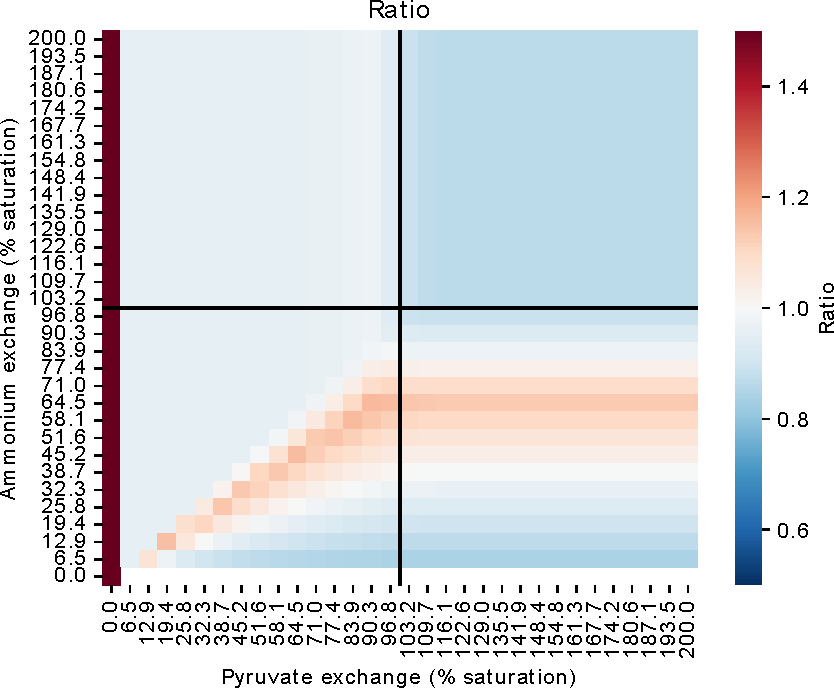
\includegraphics[width=\linewidth]{ec_grid_pyr_amm_ratio}
    \caption{
      Ratio ($\ratioabl$)
    }
    \label{fig:model-grid-pyr-ratio}
  \end{subfigure}%
  \begin{subfigure}[t]{0.45\textwidth}
  \centering
    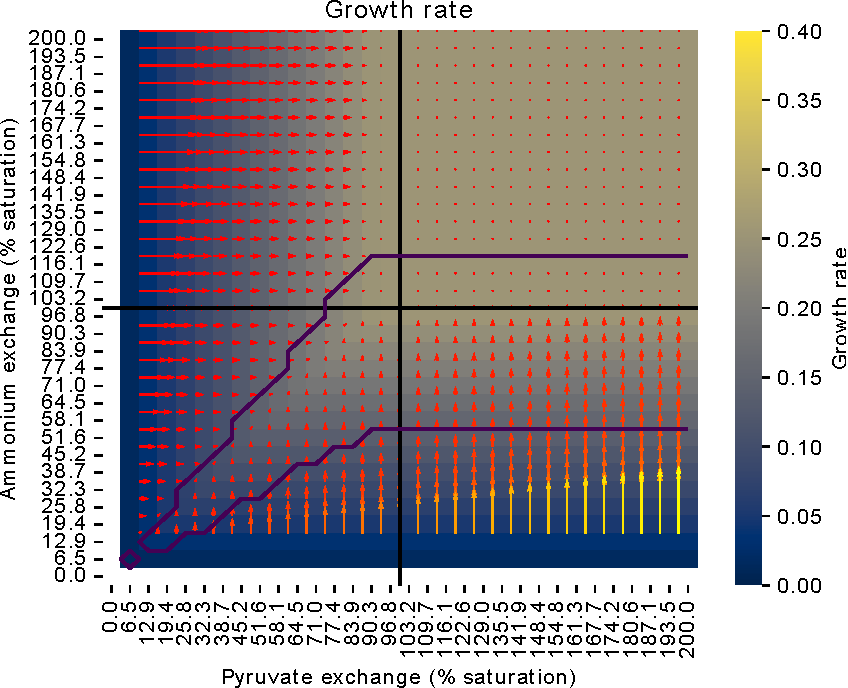
\includegraphics[width=\linewidth]{ec_grid_pyr_amm_gr}
    \caption{
      Growth rate based on unmodified biomass reaction ($\gro$)
    }
    \label{fig:model-grid-pyr-growthrate}
  \end{subfigure}

  \begin{subfigure}[t]{0.45\textwidth}
  \centering
    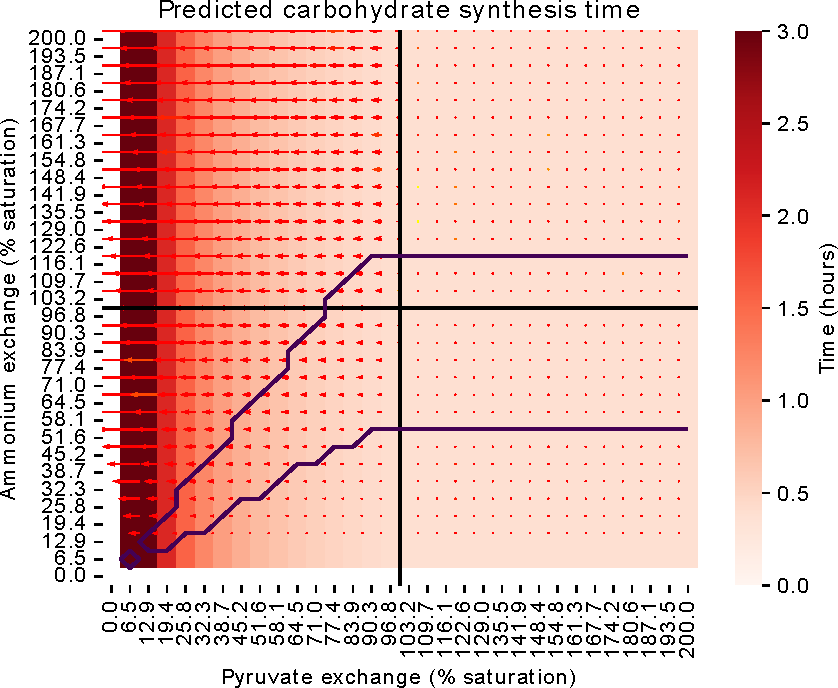
\includegraphics[width=\linewidth]{ec_grid_pyr_amm_carb}
    \caption{
      $\Tabl{carbohydrate}$
    }
    \label{fig:model-grid-pyr-carb}
  \end{subfigure}%
  \begin{subfigure}[t]{0.45\textwidth}
  \centering
    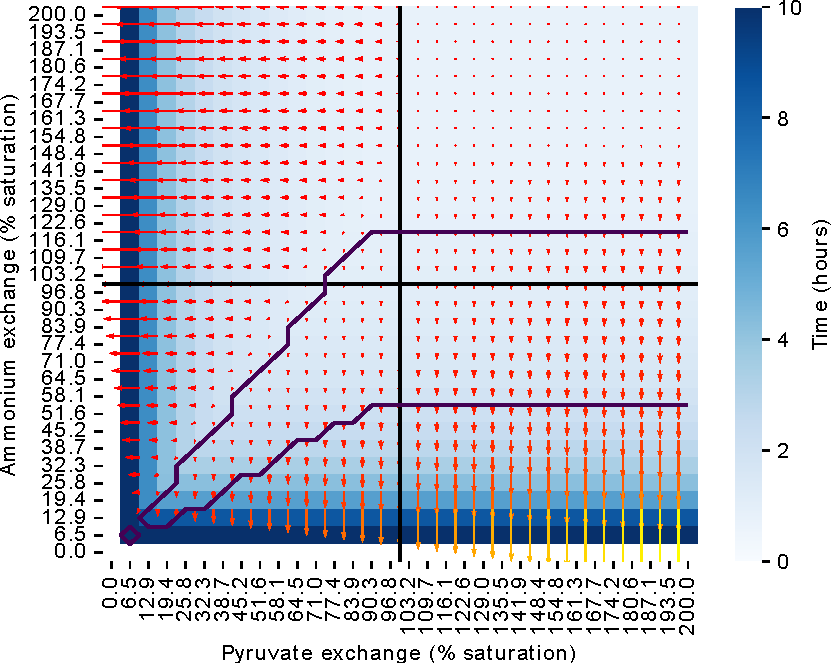
\includegraphics[width=\linewidth]{ec_grid_pyr_amm_prot}
    \caption{
      $\Tabl{protein}$
    }
    \label{fig:model-grid-pyr-prot}
  \end{subfigure}

  \begin{subfigure}[t]{0.45\textwidth}
  \centering
    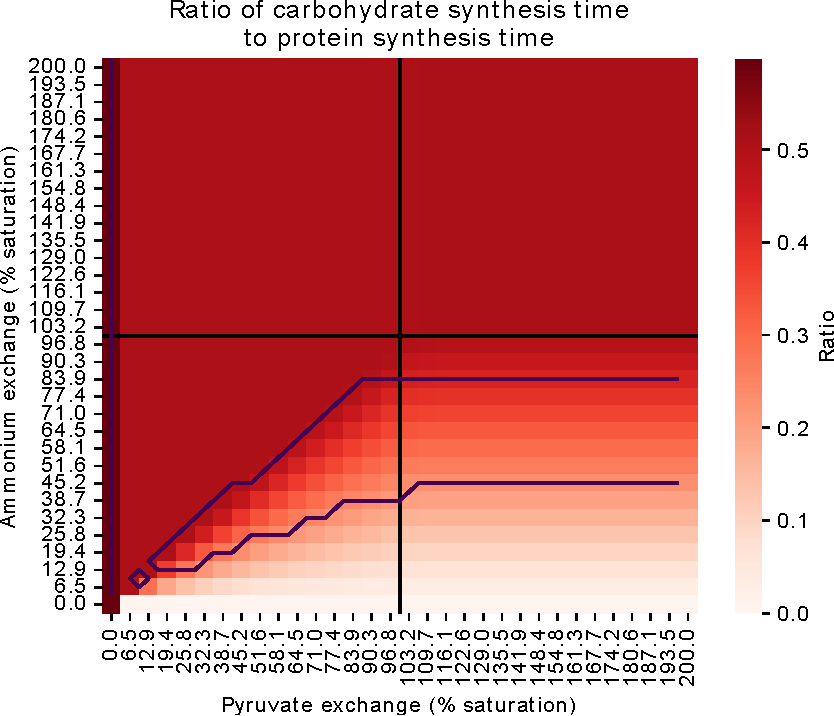
\includegraphics[width=\linewidth]{ec_grid_pyr_amm_carb_to_prot}
    \caption{
      $\Tabl{carbohydrate}/\Tabl{protein}$
    }
    \label{fig:model-grid-pyr-carb-to-prot}
  \end{subfigure}
  \caption{
    Effect of pyruvate ($\exchrate{pyruvate}$) and ammonium exchange rates ($\exchrate{ammonium}$) on various quantities.
    Exchange rates are expressed in percentages of growth saturation values shown in~\ref{fig:model-saturation}: pyruvate saturation being at \SI{4.44}{\mmolgdwh} and ammonium saturation being at \SI{1.00}{\mmolgdwh}.
    Black straight lines indicate saturation values.
    Contours show region in which ratio $\ratioabl > 1$.
    Arrows indicate susceptibility of the quantity displayed in the heatmap, relative to $\exchrate{pyruvate}$ and $\exchrate{ammonium}$.
  }
  \label{fig:model-grid-pyr}
\end{figure}

To investigate the effect on a non-fermentable carbon source, I repeated the investigation using pyruvate as the carbon source, and adjusted the saturation exchange rates accordingly: pyruvate saturation being at \SI{4.44}{\mmolgdwh} and ammonium saturation being at \SI{1.00}{\mmolgdwh} (figure~\ref{fig:model-grid-pyr}).
Overall, pyruvate seems to represent an extreme case of the glucose investigation; the changed behaviour of $\ratioabl$ with respect of pyruvate and ammonium exchange rates can be explained by a changed shape of the carbon-source saturation curve.

\begin{figure}
  \centering
  \begin{subfigure}[t]{0.45\textwidth}
  \centering
    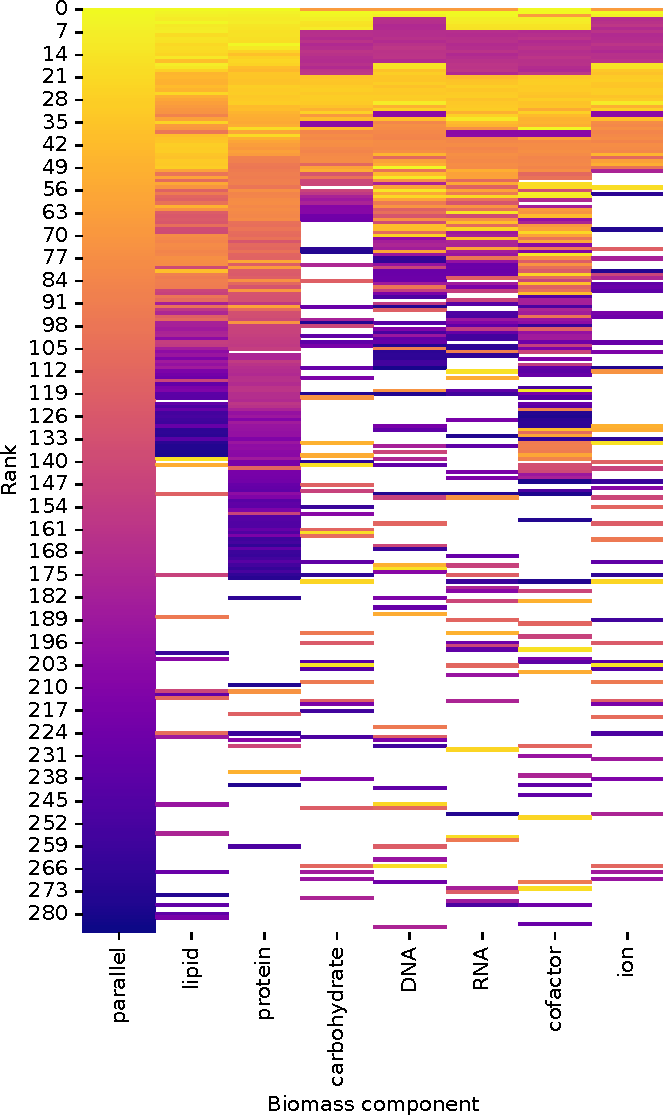
\includegraphics[width=\linewidth]{CompareEnzUse_glc16p89_pyrUnres_ammUnres_1.pdf}
    \caption{
      Rank of enzyme usage reactions in the low $\ratioabl$ case ($\exchrate{glucose}$ = \SI{16.89}{\mmolgdwh}).
    }
    \label{fig:model-rank-glc-lowratio-rank}
  \end{subfigure}%
  \begin{subfigure}[t]{0.45\textwidth}
  \centering
    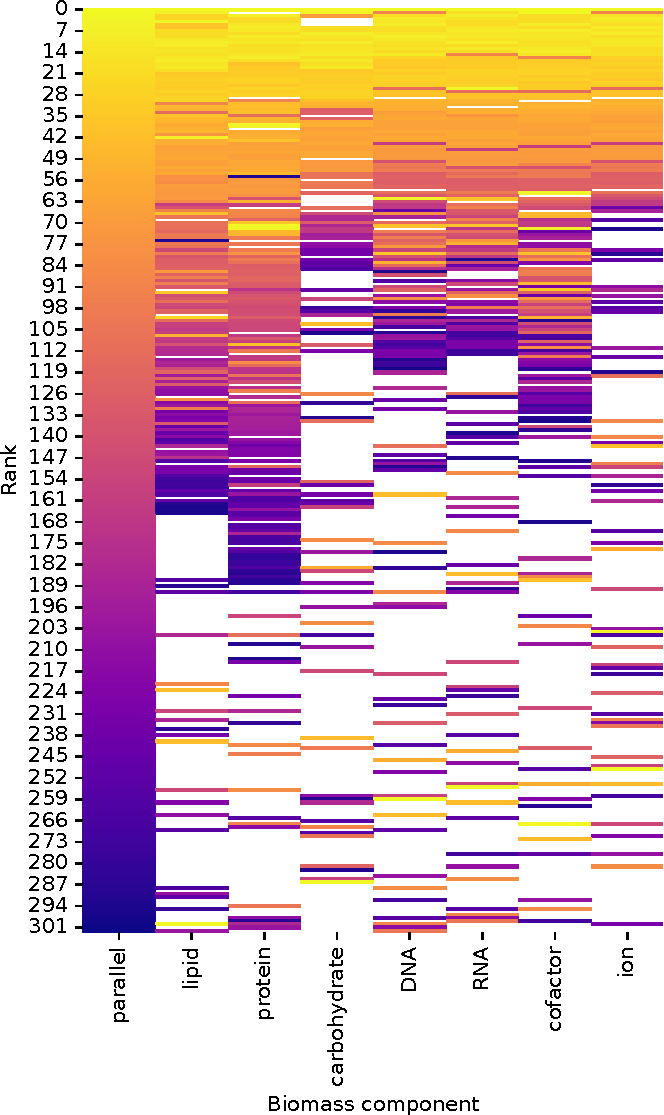
\includegraphics[width=\linewidth]{CompareEnzUse_glc01p69_pyrUnres_amm01p05_1.pdf}
    \caption{
      Rank of enzyme usage reactions in the high $\ratioabl$ case ($\exchrate{glucose}$ = \SI{1.69}{\mmolgdwh}, $\exchrate{ammonium}$ = \SI{1.05}{\mmolgdwh}).
    }
    \label{fig:model-rank-glc-highratio-rank}
  \end{subfigure}

  \begin{subfigure}[t]{0.45\textwidth}
  \centering
    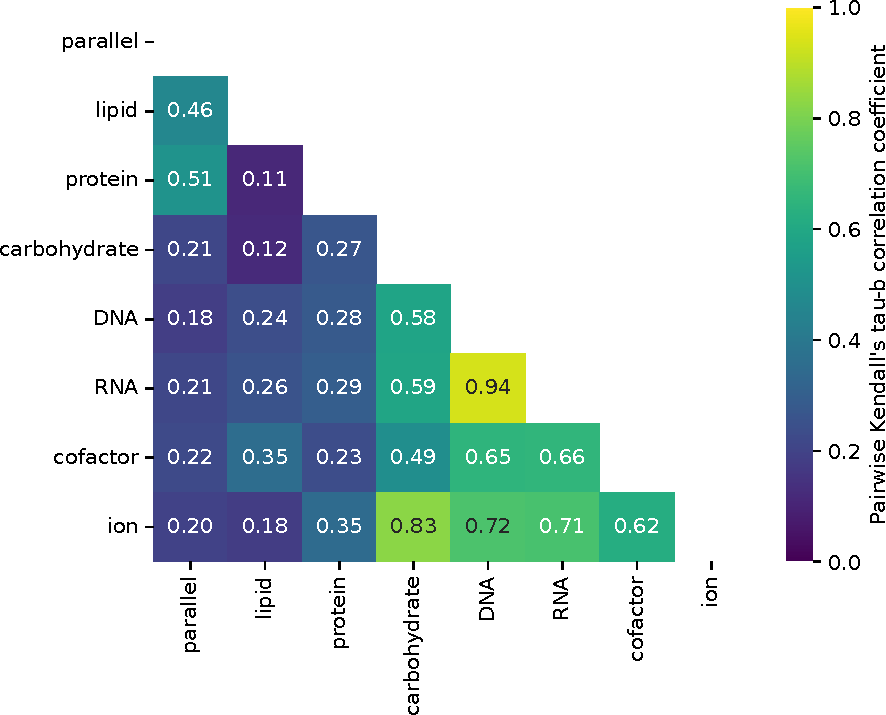
\includegraphics[width=\linewidth]{CompareEnzUse_glc16p89_pyrUnres_ammUnres_2.pdf}
    \caption{
      Pairwise Kendall's $\tau$-$b$ rank correlation coefficients for \ref{fig:model-rank-glc-lowratio-rank}.
    }
    \label{fig:model-rank-glc-lowratio-kendall}
  \end{subfigure}%
  \begin{subfigure}[t]{0.45\textwidth}
  \centering
    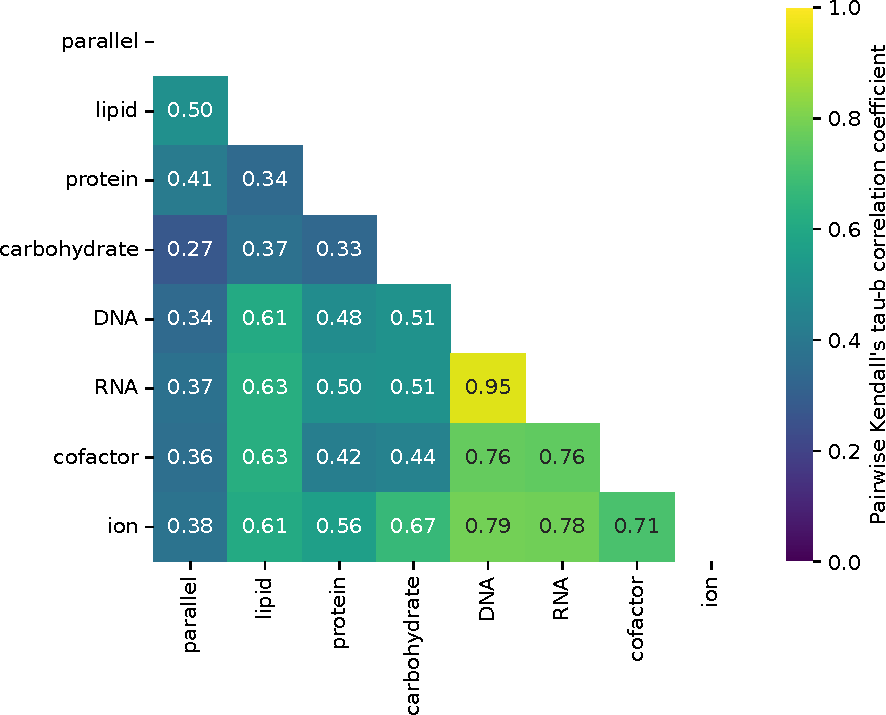
\includegraphics[width=\linewidth]{CompareEnzUse_glc01p69_pyrUnres_amm01p05_2.pdf}
    \caption{
      Pairwise Kendall's $\tau$-$b$ rank correlation coefficients for \ref{fig:model-rank-glc-highratio-rank}.
    }
    \label{fig:model-rank-glc-highratio-kendall}
  \end{subfigure}

  \caption{
    Proteome allocation favouring sequential and parallel biosynthesis strategies, with glucose as carbon source.
    \textbf{(Top panels: \ref{fig:model-rank-glc-lowratio-rank}, \ref{fig:model-rank-glc-highratio-rank})} In the parallel case (no change to biomass equation), enzyme usage reactions are ranked, in descending order, by magnitude of flux and each assigned a colour.
    When biomass components are ablated, the ranks change, as shown by how the order of colours change from column to column.
    White indicates reactions that carry zero flux in the parallel case.
    \textbf{(Bottom panels: \ref{fig:model-rank-glc-lowratio-kendall}, \ref{fig:model-rank-glc-highratio-kendall})} Kendall's $\tau$-$b$ rank correlation coefficient was computed for each pair of columns in the top panels to quantify the similarity between each case.
  }
  \label{fig:model-rank-glc}
\end{figure}

In both the glucose/ammonium and pyruvate/ammonium investigations, I observe that the highest $\ratioabl$ occurs at the boundary at which both the carbon source and the nitrogen source are limiting.
This leads to the hypothesis that the cell favours parallel biosynthesis of biomass components in such conditions, especially if the associated biomass components share metabolic pathways and if the conditions dictate similar levels of enzymes.

To evaluate this hypothesis, I investigated how the enzyme usage fluxes change across each round of ablation in the glucose/ammonium exchange combinations that produce the lowest and greatest $\ratioabl$ (figure~\ref{fig:model-rank-glc}), and performed the same investigation for pyruvate/ammonium exchange combinations (figure~\ref{fig:model-rank-pyr}).
As a visualisation aid, I ranked the enzyme usage reactions by magnitude of flux to emphasise of allocation of enzymes change in each condition, and computed the Kendall's $\tau$-b rank correlation coefficient to quantify the similarity between the enzyme usage flux vector between each pair of biomass component prioritisation situations.

Figure~\ref{fig:model-rank-glc} suggests that in the low $\ratioabl$ condition, in which both glucose and ammonium are abundant, enzyme-available proteome allocation patterns for lipid- and protein-prioritised simulations most resemble the parallel case.
In contrast, a set of enzymes that were originally synthesised in low levels in the parallel case became enzymes with the highest levels when carbohydrates, DNA, RNA, cofactors, or ions are prioritised.
This separation of biomass component-prioritised simulations into two groups according to enzyme-available proteome allocation patterns confirms the advantage of sequential biosynthesis.
Or, at least the lipids and proteins can be synthesised together, followed by the other components, or the order by which the two groups are synthesised can be reversed.
The high $\ratioabl$ condition, in which both glucose and ammonium are near-limiting, paints the opposite picture.
Here, allocation of the proteome to enzymes is similar across all situations, suggesting that parallel biosynthesis of biomass components may be advantageous in this situation.

\begin{figure}
  \centering
  \begin{subfigure}[t]{0.45\textwidth}
  \centering
    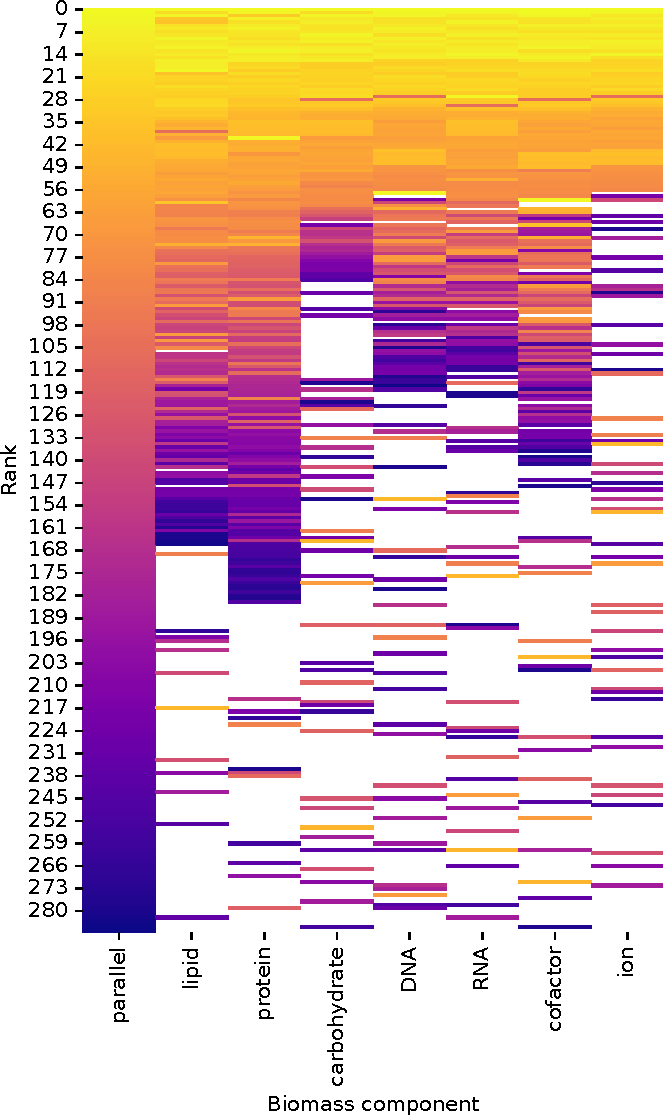
\includegraphics[width=\linewidth]{CompareEnzUse_glc00p00_pyr08p89_ammUnres_1.pdf}
    \caption{
      Rank of enzyme usage reactions in the low $\ratioabl$ case ($\exchrate{pyruvate}$ = \SI{8.89}{\mmolgdwh}).
    }
    \label{fig:model-rank-pyr-lowratio-rank}
  \end{subfigure}%
  \begin{subfigure}[t]{0.45\textwidth}
  \centering
    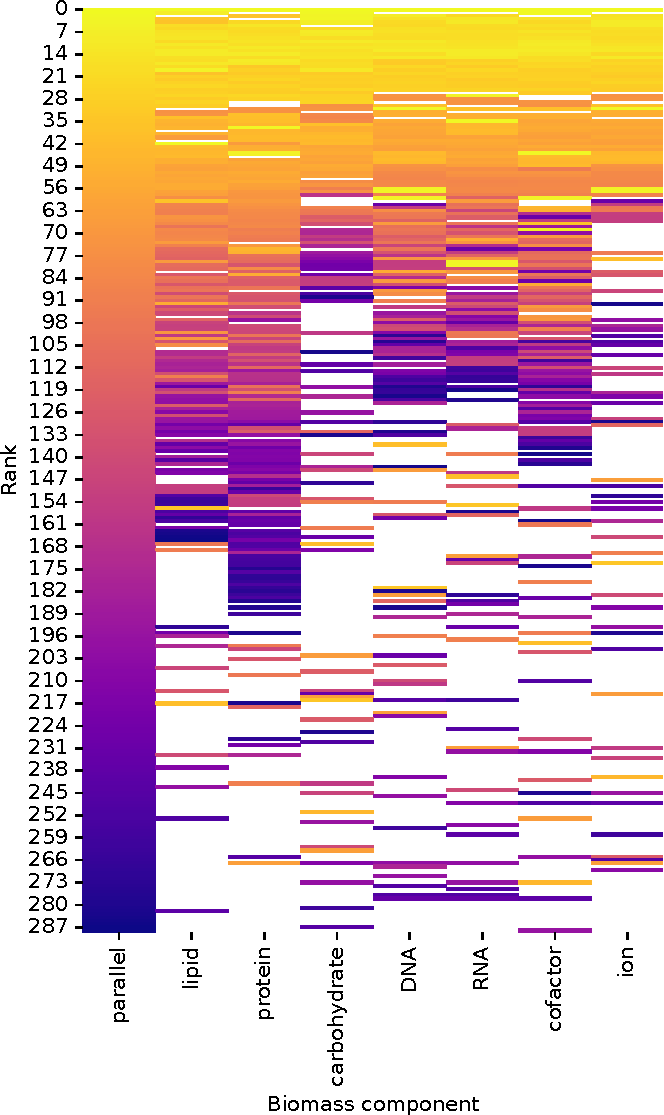
\includegraphics[width=\linewidth]{CompareEnzUse_glc00p00_pyr03p73_amm00p90_1.pdf}
    \caption{
      Rank of enzyme usage reactions in the high $\ratioabl$ case ($\exchrate{pyruvate}$ = \SI{3.73}{\mmolgdwh}, $\exchrate{ammonium}$ = \SI{0.90}{\mmolgdwh}).
    }
    \label{fig:model-rank-pyr-highratio-rank}
  \end{subfigure}

  \begin{subfigure}[t]{0.45\textwidth}
  \centering
    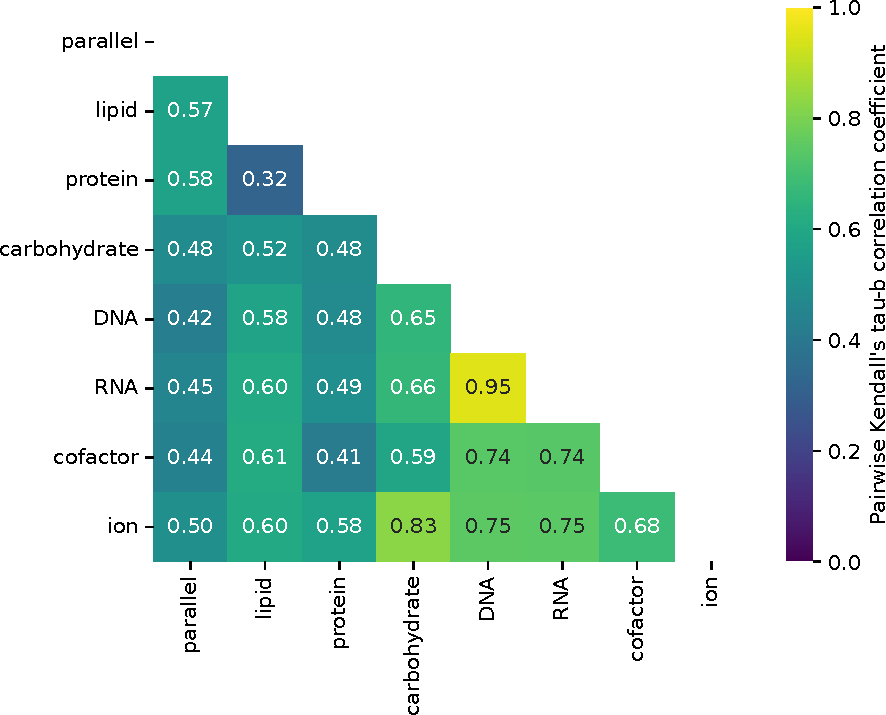
\includegraphics[width=\linewidth]{CompareEnzUse_glc00p00_pyr08p89_ammUnres_2.pdf}
    \caption{
      Pairwise Kendall's $\tau$-$b$ rank correlation coefficients for \ref{fig:model-rank-pyr-lowratio-rank}.
    }
    \label{fig:model-rank-pyr-lowratio-kendall}
  \end{subfigure}%
  \begin{subfigure}[t]{0.45\textwidth}
  \centering
    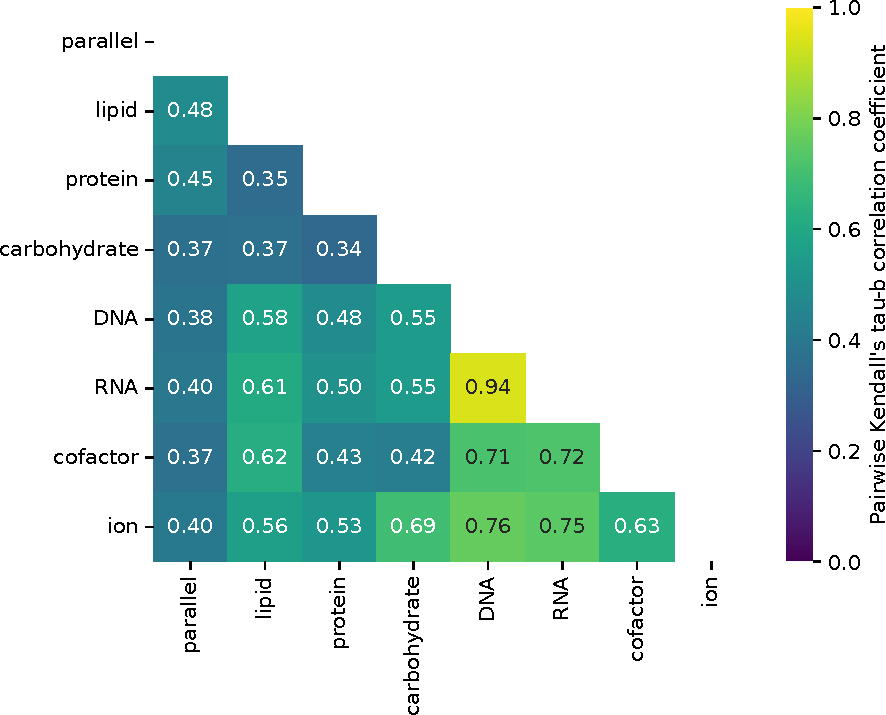
\includegraphics[width=\linewidth]{CompareEnzUse_glc00p00_pyr03p73_amm00p90_2.pdf}
    \caption{
      Pairwise Kendall's $\tau$-$b$ rank correlation coefficients for \ref{fig:model-rank-pyr-highratio-rank}.
    }
    \label{fig:model-rank-pyr-highratio-kendall}
  \end{subfigure}

  \caption{
    Proteome allocation favouring sequential and parallel biosynthesis strategies, with pyruvate as carbon source.
    \textbf{(Top panels: \ref{fig:model-rank-pyr-lowratio-rank}, \ref{fig:model-rank-pyr-highratio-rank})} In the parallel case (no change to biomass equation), enzyme usage reactions are ranked, in descending order, by magnitude of flux and each assigned a colour.
    When biomass components are ablated, the ranks change, as shown by how the order of colours change from column to column.
    White indicates reactions that carry zero flux in the parallel case.
    \textbf{(Bottom panels: \ref{fig:model-rank-pyr-lowratio-kendall}, \ref{fig:model-rank-pyr-highratio-kendall})} Kendall's $\tau$-$b$ rank correlation coefficient was computed for each pair of columns in the top panels to quantify the similarity between each case.
  }
  \label{fig:model-rank-pyr}
\end{figure}

However, figure~\ref{fig:model-rank-pyr} suggests that the contrast between each biomass component is lessened when pyruvate is the carbon source.

% Figure that shows enzyme usage fluxes being noisy may be very useful to illustrate this point...
% I can fish them from older commits (and keep the arrows).
% Also, this sentence is bloody long, but I'll deal with it in a grammar/proofreading edit.
Upon investigation of all \num{1024} nutrient conditions in each carbon source-nitrogen source pair as defined in earlier in this section, it appears that the relationship between each of the exchange rate axes and any measure of similarity between ablation rounds based on enzyme usage reactions is not continuous.
This is likely explained by the non-multiplicity of solutions in FBA.
Namely, FBA finds the optimal value of the objective function, such as growth, but the flux vector that gives rise to this objective function may differ across each simulation or each linear optimisation solver.
This is not a problem when ablation-related quantities were computed earlier in the section because they were all based on the fluxes of the objective function, defined as the biomass reaction, even if the biomass reaction itself was modified during ablation.
In other words, although choosing representative nutrient conditions leads to an attractive picture that may confirm the hypothesis of this section, the computational limitations of FBA renders any conclusion flawed.

\section{Conclusion}
\label{subsec:model-conclusion}

The identity of enzymes used during synthesis of biomass components may explain some experimental observations.
It is possible that the cell synthesises carbohydrate, DNA, and RNA after one another so that usage of  oxidative phosphorylation occur at around the same time.
This may explain cycles in dissolved oxygen concentrations.
In addition, lipid biosynthesis often requires different enzymes than the other components, and this may explain cycling of lipid stores.

Proteins are the main limiting factor for biosynthesis, mostly owing to its large mass fraction.
This is followed by carbohydrates and lipids.
However, the biosynthesis time varies significantly as the nutrient conditions vary.

The advantage of sequential biosynthesis of biomass components is retained in auxotrophs and deletion strains, confirming the robustness (presence) sequential biomass synthesis as a resource allocation strategy, and thus may explain why the metabolic cycle is still present in such strains.
It is important to note that the advantage of sequential synthesis is retained even with nutrient supplements, which ensure a good growth rate.

A smaller enzyme pool means that it is more advantageous for the cell to perform sequential biosynthesis of biomass components.

This balance between sequential and parallel synthesis of biomass components changes when nutrient conditions change --- particularly with carbon (glucose or pyruvate) and nitrogen (ammonium) source uptake changes.
In particular, it is least advantageous when both carbon and nitrogen are limiting or near-limiting (of growth rate), and is most advantageous when neither are limiting or when only ammonium is limiting.
The patterns also reflect the differing saturation patterns of glucose and pyruvate.

The degree of advantage of sequential biosynthesis in various conditions and the time scales predicted may explain why yeast cells perform metabolic cycling in certain nutrient conditions.
The model may provide a \emph{weak} explanation of why yeast cells continue to have metabolic cycles when abruptly starved of glucose.
If the glucose exchange is zero, the solution is infeasible, but if the glucose exchange is \emph{near} zero, the ratio is \emph{less than one}.
Although a better investigation would be \emph{switching} of nutrient conditions, which FBA is not built for: it only looks at steady state, and doesn't `remember' past states.

The model does not account for varying protein fractions (relative to cell dry mass) and other parameters that affect the size of $\epool$ during growth and division, and across different conditions.
For instance, \parencite{elsemmanWholecellModelingYeast2022} predicts that growth rate affects proteome fractions ($f$) and the saturation factor ($\sigma$)
However, as I find that $\epool$ affects the growth rate, there may be a circular argument here, and there is no guarantee that parameter values will converge if the cyclical effects are fully accounted for.
Furthermore, the data on biomass component fractions are old, sparse, and coarse --- as a back-of-the-envelope calculation, the model is perhaps sufficient.

In summary, results confirm temporal segregation of biosynthesis of biomass components, especially as a strategy under constraints on the size of the proteome available for the synthesis of enzymes.
Although it is unrealistic to assume that synthesis of one class macromolecule excludes all others, this approach is still instructive as it gives a back-of-the-envelope calculation to support the notion that the cell partitions biosynthesis temporally, and gives weight to the idea that this may be one of the rationale of the existence yeast metabolic cycle.

% Upon closer inspection of the times and fluxes... [INSERT RESULTS AND DISCUSSION HERE]
% - How long does it take to replicate the genome?  It is biosynthesis of nucleotides + process of polymerising them.  There has to be super basic cell division cycle literature about this...
% - Fatty acids: cell may use pentose phosphate pathway and gluconeogenesis to route flow in a cycle to generate masses of NAD(P)H.  Check if the fluxes suggest this.
